\documentclass[a4paper,fleqn,9]{ujbook}
    %========================
    % パッケージの読み込み
    %========================
      %===============================================================================
% パッケージの読み込み
%===============================================================================
%% ------------------------------------------
%% * Now Setting
%% ------------------------------------------
%\usepackage[setpagesize=false,dvipdfmx,%
%bookmarks=true,bookmarksnumbered=true,%
%bookmarksopen=false,%
%colorlinks=false,%
%pdftitle={タイトル},%
%pdfauthor={作成者},%
%pdfsubject={サブタイトル},%
%pdfkeywords={キーワード},%
%pdfborder={0 0 0},%
%linkcolor=blue,anchorcolor=blue,urlcolor=blue,
%]{hyperref}
%\RequirePackage[12tabu, orthodox]{nag}
%\usepackage{atbegshi}
%\AtBeginShipoutFirst{\special{pdf:tounicode 90ms-RKSJ-UCS2}}
%\usepackage{refcheck}              % ref auto check
\usepackage[dvipdfmx]{graphicx}
%\usepackage{mediabb}               %  pdfの図を挿入時の,大きさの設定を自動化する
%\usepackage{gradientframe}          %  図に影をつける
\usepackage[dvips]{color}           %  dvipsにて,色付文字を有効化する

\usepackage{bm}                     %  数式太字

%\usepackage{lmodern}
\usepackage{fancyhdr}

\usepackage{bbding}
\usepackage{textcomp}
\usepackage{okumacro}
\usepackage{fancybox}               %  囲みの種類の追加
%\usepackage{calrsfs}               %  文字の種類の追加 1
%\usepackage{rsfso}                 %  文字の種類の追加 2
\usepackage{ascmac}                 %  数式環境の拡張
\usepackage{amsfonts}               %  数式の拡張1
\usepackage{amsthm}                 %  数式の拡張2
\usepackage{amsmath,amssymb}        %  数式の拡張3
\usepackage{mathtools}                                %  数式の拡張4
\usepackage[sans]{dsfont}
\usepackage[T1]{fontenc}
\usepackage{pifont}
%  \mathtoolsset{showonlyrefs=true}  %    参照していない式の番号は付加しない
\usepackage{enumitem}
\usepackage[all, warning]{onlyamsmath}
%\usepackage{esvect}                %  その他のベクトル表現
\usepackage{url}                    %  \url のために必要
\usepackage{makeidx}                %  索引のために
%\usepackage{mediabb}               %  PDFファイル読み込みのために
%\usepackage[dvipdfmx]{hyperref}    %  文字化け
%\usepackage[hypertex]{hyperref}    %  動作がおかしい
\usepackage[cc]{titlepic}           %  表紙に図を挿入可能にする
%\usepackage{harmony}               %  音符が表示できるはずだが,フォントが見つからない
%\usepackage{hangcaption}           %  長いキャプションの折り返し
%\usepackage[times]{quotchap}        %  章のみだし体裁の変更
%\usepackage{pdfdraftcopy}          %  透かしを入れる
%  \draftstring{作成中}             %    -> 透かしの文字列 を設定
%\usepackage[brackets]{fnindent}    %  脚注の体裁を変更
\usepackage[version=4]{mhchem}
\usepackage{setspace}               % 行間調整してみる(\setstretch{1.5}, \begin{spacing}{0.8}-\end{spacing})
%\usepackage{breqn}                  % \begin{dmath}
\usepackage{wasysym}
\usepackage{layout}
\usepackage{braket}                 %  ディラックのブラケット
\usepackage{physics}                % 物理でよく使う数式ショートカット

\usepackage{pxrubrica}              % ルビ
\usepackage{plext}
\usepackage[T1]{fontenc}
\usepackage[utf8]{inputenc}

%\usepackage{kpfonts}
%\usepackage{txfonts}               %  Times フォントの使用
%\usepackage{newtxtext,newtxmath}   %  NewTimes フォントの使用
%\usepackage{fourier}               %  アルファベットフォント変更 1
%\usepackage{fouriernc}             %  アルファベットフォント変更 2
%\usepackage{kurier}                %  アルファベットフォント変更 3
%\usepackage{lmodern}               % Latine Modern
\usepackage{pxfonts}                %
% --- End Of Setting ---


%%%%%%%%%%%%%%%%%%%%%%%%%%%%%%%%%%%%%%%%%%%%%%%%%%%%%%%%%%%%%%%%%%%%%%%%%%%%%%%%
%%%%%%%%% Back Up Code %%%%%%%%%%%%%%%%%%%%%%%%%%%%%%%%%%%%%%%%%%%%%%%%%%%%%%%%%
%%%%%%%%%%%%%%%%%%%%%%%%%%%%%%%%%%%%%%%%%%%%%%%%%%%%%%%%%%%%%%%%%%%%%%%%%%%%%%%%
%% ------------------------------------------
%% * Old Setting (hyperref)
%% ------------------------------------------
%\usepackage[dvipdfmx,%
%colorlinks=true,%
%urlcolor=black,%
%linkcolor=black,%
%citecolor=black,%
%linktocpage=true,%
%bookmarkstype=toc,%
%bookmarksdepth=4,%
%bookmarksnumbered=true,%
%bookmarksopen=true,%
%bookmarks=true]{hyperref}
%%\AtBeginDvi{\special{pdf:tounicode EUC-UCS2}}%EUC
%\AtBeginDvi{\special{pdf:tounicode 90ms-RKSJ-UCS2}}%SJIS


    %========================
    % 表紙
    %========================
      %========================
% 表紙
%========================
    \title{
        \Huge{数学ノート 2nd}
    }

    \author{
        菅谷\;\;\;千慧
    }

    \西暦
    \date{
        \today \quad 更新\\
        {\small --> 2010年 8月 より「物理学ノート」の一部として作製開始} \\
        {\small --> 2014年 5月 より「物理学ノート」から切り出し}
    }
    % 表紙に画像を貼る
    \titlepic{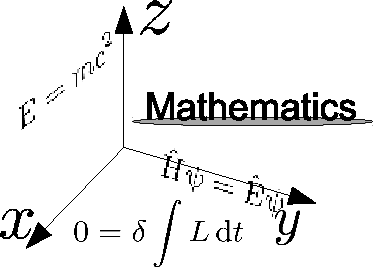
\includegraphics[keepaspectratio, width=6cm,height=3cm,clip]{hyoushi_math.pdf}}
    \par


    %========================
    % 索引作成の宣言
    %========================
      \makeindex

    %========================
    % 再定義(renewcommand)
    %========================
      %******************************************************************************
%  Newcommand
%******************************************************************************
%================================================
% * 章・節などの表示変更
%================================================
\renewcommand{\thesection}{\thechapter.\arabic{section}}
\renewcommand{\thesubsection}{\thesection.\arabic{subsection}}
\renewcommand{\tablename}{表\;}
\renewcommand{\figurename}{図\;}

\renewcommand{\bibname}{参考図書・教科書等}

%\renewcommand{\prechaptername}{第}
%\renewcommand{\postchaptername}{章}

\renewcommand{\labelenumi}{(\arabic{enumi})\;}
\renewcommand{\labelenumii}{(\alph{enumii})\;}
\renewcommand{\labelenumiii}{(\roman{enumiii})\;}
 %% - 一般の脚注のスタイル変更
%\renewcommand\thefootnote{$\mbox{}^{\clubsuit}$\kern1pt\arabic{footnote})\,} % パターン1: 三つ葉
\renewcommand\thefootnote{$\mbox{}^{\blacktriangleright}$\kern1pt\arabic{footnote})\,} % パターン2: 黒三角形
\renewcommand{\footnoterule}{%
  \vspace{1pt}                      % 線から上の幅
  \noindent\rule{0.25\textwidth}{0.5pt}   % 線の長さ,太さ
  \vspace{2pt}                     % 線から下の幅
}

\renewcommand{\textreferencemark}{\textreferencemark\,\,}
\newcommand{\komemark}{\textreferencemark}
 %% - 行間の調整
%\renewcommand{\baselinestretch}{1.05}%普通のx倍の行間間隔

%================================================
% * 演算子などの省略記述用
%================================================
% * ベクトル解析用の演算子
\newcommand{\drot}{\mathrm{rot}\,}
\newcommand{\ddiv}{\mathrm{div}\,}
\newcommand{\dgrad}{\mathrm{grad}\,}
% * ゼロベクトル
\newcommand{\bzero}{\textbf{0}}
% * 面積分
\newcommand{\sint}{\int\mspace{-11mu}\int}
% * 体積積分
\newcommand{\vint}{\int\mspace{-11mu}\int\mspace{-11mu}\int}
\newcommand{\OmegaS}{\Omega_{S}}
% * 微分記号(立った"d")
\newcommand{\df}{\,\mathrm{d}}
% * 偏微分記号
\newcommand{\rd}{\partial}
% * ダランべルシアン
\newcommand{\Dal}{\Box\,}
% * ラプラシアン
\newcommand{\Lap}{\triangle}
% * 自然対数の底
\newcommand{\e}{\mathrm{e}}
%\newcommand{\exp}{\mathrm{exp}}
% * 量子論的ハミルトニアン記号:$\qH$
\newcommand{\qH}{\mathcal{H}\,}
% * ラグランジアン密度
\newcommand{\qL}{\mathcal{L}\,}
% * 量子論的運動量演算子:$\dpx , \dpy , \dpz$
\newcommand{\dpx}{-i\hbar \frac{\partial}{\partial x}\,}
\newcommand{\dpy}{-i\hbar \frac{\partial}{\partial y}\,}
\newcommand{\dpz}{-i\hbar \frac{\partial}{\partial y}\,}
% * 量子論的エネルギー演算子:$\dE$
\newcommand{\dE}{i\hbar \frac{\partial}{\partial t}\,}
% * 量子論的ハミルトニアン演算子:$\dH$
\newcommand{\dH}{-i\hbar \nabla \,}
% * その他
\newcommand{\Shrps}{$\sharp\;$} % シャープ記号#
\newcommand{\Fig}{Fig\,\,} % 参照図を明示するときに使用する:ex.) 図\ref{xxx}
\newcommand{\Table}{図\,\,}
\newcommand{\circC}{${}^{\circ}$C}

%================================================
% * 標準的な画像のサイズ
%================================================
% 4:3 Default Size
\newcommand{\includegraphicsdefault}[1]{\includegraphics[keepaspectratio, width=4.00cm, height=3.00cm, clip]{#1}}
% 4:3 Middle Size
\newcommand{\includegraphicsmiddle}[1]{\includegraphics[keepaspectratio, width=6.00cm, height=4.5cm, clip]{#1}}
% 4:3 Large Size
\newcommand{\includegraphicslarge}[1]{\includegraphics[keepaspectratio, width=7.2cm, height=4.98cm, clip]{#1}}
% 2:1 Default Size
\newcommand{\includegraphicshalfmid}[1]{\includegraphics[keepaspectratio, width=6cm, height=3cm, clip]{#1}}
% 1:1 Squeare Default Size
\newcommand{\includegraphicssqmid}[1]{\includegraphics[keepaspectratio, width=4.00cm, height=4.00cm, clip]{#1}}
% 1:1 Squeare Default Size
\newcommand{\includegraphicssqmlrg}[1]{\includegraphics[keepaspectratio, width=7.2cm, height=7.2cm, clip]{#1}}

% Two Graphics Size
\newcommand{\includegraphicsdouble}[1]{\includegraphics[keepaspectratio, width=3.2cm, height=2.4cm, clip]{#1}}


%================================================
% * アルファベットの太字(ベクトルとか)
%================================================
\newcommand{\ba}{\boldsymbol{a}}
\newcommand{\bb}{\boldsymbol{b}}
\newcommand{\bc}{\boldsymbol{c}}
\newcommand{\bd}{\boldsymbol{d}}
\newcommand{\be}{\boldsymbol{e}}
\newcommand{\bg}{\boldsymbol{g}}
\newcommand{\bldf}{\boldsymbol{f}}
\newcommand{\bj}{\boldsymbol{j}}
\newcommand{\bp}{\boldsymbol{p}}
\newcommand{\br}{\boldsymbol{r}}
\newcommand{\bv}{\boldsymbol{v}}
\newcommand{\bx}{\boldsymbol{x}}
\newcommand{\by}{\boldsymbol{y}}
\newcommand{\bz}{\boldsymbol{z}}
\newcommand{\bn}{\boldsymbol{n}}
\newcommand{\bE}{\boldsymbol{E}}
\newcommand{\bF}{\boldsymbol{F}}
\newcommand{\bC}{\boldsymbol{C}}
\newcommand{\bB}{\boldsymbol{B}}
\newcommand{\bA}{\boldsymbol{A}}
\newcommand{\bi}{\boldsymbol{i}}
\newcommand{\bt}{\boldsymbol{t}}
\newcommand{\bk}{\boldsymbol{k}}
\newcommand{\bl}{\boldsymbol{l}}
\newcommand{\bS}{\boldsymbol{S}}
\newcommand{\bI}{\boldsymbol{I}}
\newcommand{\bH}{\boldsymbol{H}}
\newcommand{\bP}{\boldsymbol{P}}
\newcommand{\bD}{\boldsymbol{D}}
\newcommand{\bX}{\boldsymbol{X}}
\newcommand{\bY}{\boldsymbol{Y}}
\newcommand{\bL}{\boldsymbol{L}}
\newcommand{\bM}{\boldsymbol{M}}
\newcommand{\bN}{\boldsymbol{N}}
\newcommand{\bo}{\boldsymbol{o}}
\newcommand{\bU}{\boldsymbol{U}}
\newcommand{\bV}{\boldsymbol{V}}
\newcommand{\bW}{\boldsymbol{W}}
\newcommand{\bZ}{\boldsymbol{Z}}
\newcommand{\setN}{\mathbb{N}}
\newcommand{\setC}{\mathbb{C}}
\newcommand{\setZ}{\mathbb{Z}}
\newcommand{\setR}{\mathbb{R}}
\newcommand{\setA}{\mathbb{A}}
\newcommand{\setB}{\mathbb{B}}
\newcommand{\setD}{\mathbb{D}}
\newcommand{\setE}{\mathbb{E}}
\newcommand{\setF}{\mathbb{F}}
\newcommand{\bldi}[1]{\textit{\textbf{{#1}}}}
\newcommand{\bld}[1]{\textbf{{#1}}}

%================================================
% * 花文字
%================================================
\newcommand{\flwA}{\mathcal{A}}
\newcommand{\flwB}{\mathcal{B}}
\newcommand{\flwC}{\mathcal{C}}
\newcommand{\flwD}{\mathcal{D}}
\newcommand{\flwE}{\mathcal{E}} % 起電力
\newcommand{\flwF}{\mathcal{F}} % 一般化された力とか
\newcommand{\flwH}{\mathcal{H}} %
\newcommand{\flwp}{\mathcal{p}} % 一般化された運動量
\newcommand{\flwL}{\mathcal{L}}

%================================================
% * ギリシア数字作成
%================================================
\newcommand{\I}{I}
\newcommand{\II}{I\hspace{-.1em}I}
\newcommand{\III}{I\hspace{-.1em}I\hspace{-.1em}I}
\newcommand{\IV}{I\hspace{-.1em}V }
\newcommand{\V}{V}
\newcommand{\VI}{V\hspace{-.1em}I}
\newcommand{\VII}{V\hspace{-.1em}I\hspace{-.1em}I}
\newcommand{\VIII}{V\hspace{-.1em}I\hspace{-.1em}I\hspace{-.1em}I }
\newcommand{\X}{X}
%再定義1(数式番号の表現 chap-sub-subsub)
%\makeatletter
% \renewcommand{\theequation}{%
  % \thesection.\arabic{equation}}
  %\@addtoreset{equation}{section}
 %\makeatother

%================================================
% * 新しいカウンタの生成
%================================================
% * 宣言
\newcounter{Memo}           %
\newcounter{Snumber}        % "memo" の番号
\newcounter{myshade}        % 物理部分の重要事項の番号
\newcounter{PreAttentionNo} % 記入方法の諸注意の番号
\newcounter{AboutThisNoteNo}% 「このノートにいて」の番号
% * 初期値設定
\setcounter{Memo}{1}
\setcounter{Snumber}{1}
\setcounter{myshade}{1}
\setcounter{PreAttentionNo}{1}
\setcounter{AboutThisNoteNo}{1}

%================================================
% * カウンタの再設定
%================================================
% * 目次の表示の深さを設定する
\setcounter{secnumdepth}{6}
\setcounter{tocdepth}{4}
% * 立て揃え で改行を許す:0から4まで
%    0      ; 絶対改行しない
%    1から3 ; 適度に改行する.数字が高いほど,
%             基準が緩くなる
%    4      ; 必ず改行する
\allowdisplaybreaks[4]

%================================================
% 図のcaptionの : をとる
%================================================
\makeatletter
\long\def\@makecaption#1#2{%
\vskip\abovecaptionskip%
%\sbox\@tempboxa{#1: #2}% <--- original
\sbox\@tempboxa{#1\;\; #2}
\ifdim \wd\@tempboxa >\hsize%
%#1: #2\par <--- original
#1 #2\par
\else
\global \@minipagefalse
\hb@xt@\hsize{\hfil\box\@tempboxa\hfil}%
\fi
\vskip\belowcaptionskip}
\makeatother
%------------------------------------------------

%******************************************************************************
%  Newtheorem
%******************************************************************************
%定義や定理の出力は,newtheorem 環境を使用します.
%定義の場合,プリアンブルに次の内容を記述します.
%
%\newtheorem{dfn}{Definition}[引数]

%「定義」と表示させたい場合は,
%Definition を 定義 に書き換えます.
%
%定義番号に (2.1) のように章番号をつけたい場合は,
%引数に,[chapter]を入力します.
%章立ての文書で (1.3.2) のように節番号を付けたい場合は,
%引数にsection を入力します.
%
%% 使い方:定理の場合
%\begin{thm}
%集合 $A, B$ について,$A$ から $B$ への単射および $B$ から $A$ への単射がともに
%存在すれば,$A$ と $B$ の濃度が等しい.
%\end{thm}
\theoremstyle{plain}
\newtheorem{thm}{定理}[section]
\newtheorem{lem}{補題}[section]
\newtheorem{cor}{系}[section]
\newtheorem{prp}{命題}[section]
%
\theoremstyle{definition}
\newtheorem{dfn}{定義}[section]
%
\theoremstyle{remark}
\newtheorem{rem}{注意}
\newtheorem{prf}{証明}

%******************************************************************************
% Newenvironment
%******************************************************************************
% * Environment: \memo
\newenvironment{memo}[1]
{ % before
    \addcontentsline{toc}{subsubsection}{\Shrps\textit{memo} No.\theSnumber : #1} % 目次
    \subsubsection*{\Shrps\textit{memo} No.\theSnumber : \emph{#1}}
    %\addcontentsline{toc}{subsubsection}{\;\;\;\Shrps\textit{memo} \; #1}
    %\subsubsection*{\;\;\;\Shrps\textit{memo} \;\;\; \emph{#1}}
    \stepcounter{Snumber}
    \small
}
{ % after
    \par \normalsize
}

% * Environment: \myshadebox
\newenvironment{myshadebox}[1]
{ % before
    %\addcontentsline{toc}{subsubsection}{\;\S\;Point No.\themyshade :\; #1} % 目次
    \leavevmode \\  \leavevmode \\
    \begin{shadebox}
        %\;\textbf{\ding{42}\;Point No.\themyshade :\, #1} \leavevmode \\
                \textbf{\;Point \themyshade :\, \textbf{#1}} \vspace{1mm} \\
        \leavevmode
        \stepcounter{myshade}
}
{ % after
    \end{shadebox}
    \leavevmode \\
}

% * Environment: \comment
\newenvironment{mycomment}
{ % before
    \par \small
    \textbf{コメント$\quad$}
}
{ % after
    \newline \par \normalsize
}

% * Environment: \mysmallsec
\newenvironment{mysmallsec}[1]
{ % before
%    \addcontentsline{toc}{subsubsection}{\$ #1} % 目次
%    \subsubsection*{\$ #1}
    \subsubsection*{\P \; #1}
}

% * Environment: \pre_attention
\newenvironment{preattention}[1]
{ % before
    \addcontentsline{toc}{section}{(\thePreAttentionNo) #1} % 目次
    \subsubsection*{(\thePreAttentionNo) \emph{#1}}
    \stepcounter{PreAttentionNo}
    \label{my:preattention:#1}
}
{ % after
}

% * Environment: \aboutthisnote
\newenvironment{aboutthisnote}[1]
{ % before
    %\addcontentsline{toc}{section}{\$\theAboutThisNoteNo #1} % 目次
    \subsubsection*{\$\theAboutThisNoteNo \emph{#1}}
    \stepcounter{AboutThisNoteNo}
    \small
}
{ % after
    \par \normalsize
}
%独自コマンドの設定・既存コマンド変更の設定

    %========================
    % テキストレイアウト
    %========================

%テキストレイアウトの設定====================
    %******************************************************************************
%  TeX Layout ( A4 Paper version )
%******************************************************************************
%数式のフォントの選択
%\usepackage{txfonts}
%\usepackage{pxfonts}
%\usepackage[T1]{fontenc}
%\usepackage{lmodern}

%英文文字フォントの選択
%\usepackage{timesnew} %Times new Roman

%ページ番号全体の非表示化
%\pagestyle{empty}

%文書レイアウト
\setlength{\topmargin}{-10mm}
\setlength{\textwidth}{155mm}
\setlength{\textheight}{256mm}
\setlength{\oddsidemargin}{15mm}
\setlength{\evensidemargin}{-10mm}
        %フッタ,ヘッダと本文との行間の調整
\setlength{\headsep}{2zw}
\setlength{\footskip}{1zw}

\setlength{\parindent}{1zw} % 段落先頭のスペース zw...全角1文字単位
\setlength{\parskip}{0.4zw} % 段落間スペース

%\renewcommand{\baselinestretch}{0.9}%普通のx倍の行間間隔
%\raggedbottom

%テキストのレイアウトの設定
%=======================================

%%*=*=*=*=*=*=*=*=*=*=*=*=*=*=*=*=*=*=*=*=*=*=*=*=*=*=*=*=*=*=*=*=*=*=*=*=*=*%%
%%                             本             文
%%*=*=*=*=*=*=*=*=*=*=*=*=*=*=*=*=*=*=*=*=*=*=*=*=*=*=*=*=*=*=*=*=*=*=*=*=*=*%%
\begin{document}

    %========================
    % 前処理
    %========================
      
    %===========================================================================
    % * 表紙作成
    %===========================================================================
        \maketitle
        \pagenumbering{roman} %ページ番号の数字をローマ数字にする
        \setcounter{page}{2}  %表紙のじベージに空白ページ挿入
%%
%%    %===========================================================================
%%    % * まえおき「このノートについて」の挿入
%%    %===========================================================================
%%        \frontmatter %まえおきであることの宣言
%%        \addcontentsline{toc}{chapter}{\textbf{このノートについて}}
%%        \section*{このノートについて}
\begin{aboutthisnote}{作成方法}
    \textbf{このノートの作成にはp\LaTeXe を使用させて頂きました}.
\end{aboutthisnote}

\begin{aboutthisnote}{作成動機}
    このノートを作ることにしたのは,
    将来の自分のためです.おそらく,
    今学習している『物理学』の内容を
    忘れてしまっていると思うので,
    その記録をしておこうというものです.
\end{aboutthisnote}

\begin{aboutthisnote}{内容についての重要な注意}
    このノートの内容は
    教科書を読んだ直後に
    書いたものなので,
    教科書の内容そのままである部分が大半です.
    つまり,私のオリジナルではなく,
    様々な教科書をつぎはぎしたものです.
    しかし,(一部の引用を除いて)教科書の丸写しではなく,私なりにその内容を
    解釈して記述していますので,その教科書の内容の正確さが失われてる
    可能性があります.
    何か変な点,矛盾する箇所等があった場合は,
    すぐにその内容を修正するようにして下さい.
\end{aboutthisnote}

\begin{aboutthisnote}{言い訳}
    物理学は教科書がたくさんあり,
    また,趣味で物理学をなさっていて
    Websiteを開いている方々も多いです.
    このノートの内容はほとんどが教科書やWebによるものです.
    しかしそれでも,人から聞いたり本で読んだりした知識ではありますが,
    その知識を自分なりにノートという形でまとめることで自分の中で再定式化できれば,
    新しいものの見方を発見できるかもしれないと思い本ノートの作成を続けています.
\end{aboutthisnote}

\begin{aboutthisnote}{補足}
    このノートは物理学の理論だけを記述しており,その具体的なことは書いていないことが多いです.
    具体例を考えることで,その法則の意味をより深く理解することができますが,
    具体例は割愛しています.しかし,書かないからといって,重要でないということでは決してありません.
    具体的な問題を演習することは,例えば,定義された物理量の
    直感的な把握や,大体の大きさの見当をつけるのに役に立ちます.また,
    複数の法則の結びつき方を感じ取ることもできます.
    従って,具体例は必ず演習書等を用いて,考えなければいけません.
    理論だけ読んでいても,本当にその理論が現実と一致するかどうかは,多くの場合,
    演習を通してでしか確認できません.
    学校や科学館などでもない限り,実験して確かめるということは難しいことが多いのです.
    まあ,理論を読んで満足ができるわけがないことは当たり前なのですが(法則の現実性を
    “実感”しない限り,その法則は私にとって,確かなものではないから),
    演習をおろそかにしがちな自分に注意するために,ここに書いておきました.
\end{aboutthisnote}

\begin{aboutthisnote}{挿入図について}
    図の多くは,寺嶋容明さん
    の作られた「EPS-draw」を用いて,私が作図したものです.
    また,LibreOfficeのDrawで作図したものもあります.
    グラフの作成は,PerlやPythonにより数値計算をして,
    LibreOfficeのcalcで図式化しています.
    gnuplotで書いたところもあります.
    曲面の作成にはフリーの数式処理ソフトmaximaを使って作成
    しているところもあります.
\end{aboutthisnote}

\begin{aboutthisnote}{内容を鵜呑みにしないで下さい}
    このノートはド素人が書いたものであり,正確である保証はありません.
    むしろ,間違っている所があることは確実でしょう.
    特に,計算ミスに不安を感じます.見つけ次第,訂正していきます.
\end{aboutthisnote}

\begin{aboutthisnote}{これはノートです}
    このノートは教科書風の体裁を取っていますが,あくまでも学習ノートです.
    従って,項目の配置は論理的ではありません.メモ書き程度のものです.
\end{aboutthisnote}

\begin{aboutthisnote}{記載順}
    物理学の内容を学習する目的で,このノートをはじめから読もうとしても,
    その内容に行き着くまでには時間がかかることと思います.
    数学の学習と物理学の考え方などが,物理学の前提知識として,先立って
    説明されているからです.
    なので,そういった読み方をしてしまうと,挫折してしまうでしょう.
    このノートの使い方として,まずは目次をみて,参照したい部分を
    見つけて読む,という方法が良いと思います.
\end{aboutthisnote}

\begin{aboutthisnote}{記述精神}
    できるだけ,詳しく書こうと思います.式変形も省略なしにしたいです.
    さらにできることなら,将来,このノートを参考に,理解した物理学を論理的に自身の
    中で再構成した文書を作りたいです.
\end{aboutthisnote}

\begin{aboutthisnote}{脚注の多さについて}
    ノートを記載していた時の心境を脚注に書いておく.
    あとで,なんでそのような記述をしたかを思い起こすヒントになるはず.
    脚注が多すぎて読みにくくなってしまうが,ノートなのでいくら汚く
    書いてもOKとしたい.
\end{aboutthisnote}

\begin{aboutthisnote}{願望}
    私は,物理学を“習得”しようとは考えていません.私にとって物理学の学習は趣味です.
    物理学を勉強する理由は,それを使えるようにするためではなく,物理法則を知りたいからです.
    自然はどのように成立しているのか.自分なりに,物理学を実感したいのです.
    ですので,このノートは単に物理学の表面しか,記述していません
        \footnote{
            もしかしたら,表面もすらも記述していないかもしれない,という不安があります.
        }.

    このノートを書くことが生涯の趣味になることを期待しています.
\end{aboutthisnote}

%%%%\begin{aboutthisnote}{このノートの目標}
%%%%    最後に,学習のひそかな到達目標について.このノートの到達
%%%%    目標を“超電導”にしたいと考えています.卒研の内容が超電導現象に
%%%%    関する実験的なことだったので,理論的な事も知りたいからです.
%%%%    ただ,超電導はとても難しいので,そこに到達できるかどうかは
%%%%    わかりません...
%%%%
%%%%    また,パソコンの動作を物理学から理解したいという願望(私にとっては野望)もある.
%%%%
%%%%\end{aboutthisnote}

    以下,文の読みやすさと文字数のことを考えて,丁寧語による記述をやめます.

%%
%%    %===========================================================================
%%    % * まえおき「このノートで使用する記号」の挿入
%%    %===========================================================================
%%        \newpage
%%        \addcontentsline{toc}{chapter}{\textbf{このノートで使用する記号}}
%%        \section*{このノートで使用する記号}
    このノートで使用する記号について,
    以下に示しておく.
    ノートを読んでいて分からくなった記号
    があったら,これを参考にしてもらいたい.
    もちろん,用語については本文を参照にすること.

    複数の意味で使われる記号がいくつもあるが,
    それらについてはスラッシュ / で区切りをいれた.

    % [約束] 一行に収まる程度(30文字程度)で説明すること(体裁のため)

    %===========================================================
    % * アルファベット(斜太字:大文字)
    %===========================================================
    \subsubsection*{アルファベット(太字:大文字)}
    \begin{tabular}{lll}
        $\bE$                   &:  & 電場                                                                  \\
        $\bA$                   &:  & ベクトルポテンシャル                                                  \\
        $\bB$                   &:  & 磁束密度                                                              \\
        $\bI$                   &:  & 電流                                                                  \\
        $\bD$                   &:  & 電束密度                                                              \\
        $\bH$                   &:  & 磁場                                                                  \\
        $\bP$                   &:  & 誘電分極                                                              \\
        $\bL$                   &:  & 角運動量                                                              \\
        $\bN$                   &:  & 回転力(トルク)                                                      \\
        $\bF$                   &:  & 力(合成力)                                                          \\
        $\bM$                   &:  & 磁化                                                                  %\\
    \end{tabular}

    %===========================================================
    % * アルファベット(斜太字:小文字)
    %===========================================================
    \subsubsection*{アルファベット(太字:小文字)}
    \begin{tabular}{lll}
        $\br$                   &:  & 位置,$(\,x,\,y,\,z\,)$ と同じ.                                      \\
        $\bv$                   &:  & 速度,$(\,v_{x},\,v_{y},\,v_{z}\,)$ と同じ                            \\
        $\ba$                   &:  & 加速度,$(\,a_{x},\,a_{y},\,a_{z}\,)$ と同じ                          \\
        $\bp$                   &:  & 運動量,$(\,p_{x},\,p_{y},\,p_{z}\,)$ と同じ                          \\
        $\bi$                   &:  & 電流密度,$(\,i_{x},\,i_{y},\,i_{z}\,)$ と同じ                        \\
        $\bldf$                 &:  & 分解された力                                                          %\\
    \end{tabular}

    %===========================================================
    % * アルファベット(斜細字:大文字)
    %===========================================================
    \subsubsection*{アルファベット(細字:大文字)}
    \begin{tabular}{lll}
        $G$                     &:  & 万有引力定数,または,重力定数                                        \\
        $U$                     &:  & ポテンシャルエネルギー                                                \\
        $T$                     &:  & 運動エネルギー/張力                                                   \\
        $E$                     &:  & 全エネルギー/電場の大きさ                                      \\
        $U$                     &:  & ポテンシャル/内部エネルギー                                 \\
        $L$                     &:  & 角運動量/ラグランジアン                                               \\
        $I$                     &:  & 力積/電流の大きさ                                              \\
        $S$                     &:  & 面積/任意の閉曲面                                                     \\
        $V$                     &:  & 体積                                                                  \\
        $O$                     &:  & 原点                                                                  \\
        $H$                     &:  & ハミルトニアン/磁場の大きさ                            %\\
    \end{tabular}

    %===========================================================
    % * アルファベット(斜細字:小文字)
    %===========================================================
    \subsubsection*{アルファベット(細字:小文字)}
    \begin{tabular}{lll}
        $l$                     &:  & 長さ/任意の閉曲線                                                     \\
        $m$                     &:  & 質量(慣性質量と重力質量)                                                   %\\
    \end{tabular}

    %===========================================================
    % * アルファベット(添字付き)
    %===========================================================
    \subsubsection*{アルファベット(添字付き)}
    \begin{tabular}{lll}
        $m_{\mathrm{i}}$        &:  & 慣性質量                                                              \\
        $m_{\mathrm{g}}$        &:  & 重力質量                                                              \\
        $S_{l}$                 &:  & 任意の閉曲線 $l$ を縁とする曲面                   \\
        $k_{B}$                 &:  & ボルツマン定数                                                        %\\
    \end{tabular}

    %===========================================================
    % * アルファベット(立太字:大文字)
    %===========================================================

    %===========================================================
    % * アルファベット(立太字:小文字)
    %===========================================================

    %===========================================================
    % * アルファベット(立細字:大文字)
    %===========================================================
    \subsubsection*{アルファベット(立細字:大文字)}
    \begin{tabular}{lll}
        K                       &:  & 任意の慣性系                                                          \\
        K$'$                    &:  & Kとは別の任意の慣性系                                                 %\\
    \end{tabular}

    %===========================================================
    % * アルファベット(立細字:小文字)
    %===========================================================

    %===========================================================
    % * 花文字
    %===========================================================
    \subsubsection*{花文字}
    \begin{tabular}{lll}
        $\qL$                   &:  & ラグランジアン密度                                                    \\
        $\qH$                   &:  & 量子論ハミルトニアン演算子                                            \\
        $\flwF$                 &:  & 一般化された力                                                        \\
        $\flwE$                 &:  & 起電力                                                                %\\
    \end{tabular}

    %===========================================================
    % * ギリシア文字(大文字)
    %===========================================================
    \subsubsection*{ギリシア文字(大文字)}
    \begin{tabular}{lll}
        $\Sigma$                &:  & 総和の記号                                                            \\
        $\Omega$                &:  & 任意の領域の内部                                 %\\
    \end{tabular}

    %===========================================================
    % * ギリシア文字(小文字)
    %===========================================================
    \subsubsection*{ギリシア文字(小文字)}
    \begin{tabular}{lll}
        $\gamma$                &:  & ローレンツ因子                                                        \\
        $\nu$                   &:  & 周波数                                                                \\
        $\rho$                  &:  & 電荷密度/電気抵抗率                                                   \\
        $\sigma$                &:  & 電気伝導率                                                            \\
        $\phi$                  &:  & 電気的なポテンシャルエネルギー                                        %\\
    \end{tabular}

    %===========================================================
    % * ギリシア文字(添字付き)
    %===========================================================
    \subsubsection*{ギリシア文字(添字付き)}
    \begin{tabular}{lll}
        $\Omega_{S}$            &:  & 任意の閉曲面の内側の領域                         %\\
    \end{tabular}

    %===========================================================
    % * 数式記号
    %===========================================================
    \subsubsection*{数式記号の意味}
    $\bA$,$\bB$ は一般の(特に意味を与えない)ベクトルであるとする.
    $\br$ は位置ベクトル,$\bt$ は線素ベクトル,$\bS$ は面素ベクトルとする.
    また,$f(x)$ は $x$ を独立変数とする一次関数であり,
    $f(x,\,y,\,\cdots)$ は $(x,\,y,\,\cdots)$ を独立変数とするとする多変数関数である.\\

    \begin{tabular}{lll}
            $\bA \perp \bB$                                         &:  & $\bA$ は $\bB$ に \textbf{垂直}                          \\
            $\bA \parallel \bB$                                     &:  & $\bA$ は $\bB$ に \textbf{平行}                          \\
            $\bA_{\perp \bB}$                                       &:  & $\bA$ の $\bB$ に \textbf{垂直な成分}                    \\
            $\bA_{\parallel \bB}$                                   &:  & $\bA$ の $\bB$ に \textbf{平行な成分}                    \\
            $\displaystyle \int f(x) \df x$                         &:  & 積分         \\
            $\displaystyle \oint f(\br) \cdot \df \bt$              &:  & 線積分        \\
            $\displaystyle \sint f(\br) \cdot \df \bS$              &:  & 面積分        \\
            $\displaystyle \vint f(\br) \df V$                      &:  & 体積積分      \\
            $\df f$                                                 &:  & 微分/全微分     \\
            $\displaystyle \frac{\df}{\df x} f(x)$                  &:  & 導関数          \\
            $\displaystyle \frac{\rd}{\rd x} f(x,\, y,\, \cdots)$   &:  & 偏微分      \\
    \end{tabular}

    %===========================================================
    % * 行内に書く場合の,演算子について
    %===========================================================
    \subsubsection*{行内に書く場合の演算子の形}
        \begin{tabular}{lll}
            $ab/cd$                 &:  & $\displaystyle \frac{ab}{cd}$ を文中で記す場合.            \\
            $(a/b)(c/d)$            &:  & $\displaystyle \frac{a}{b}\frac{c}{d}$ を文中で記す場合.   \\
            $\sum_{n=1}^{N}$        &:  & $\displaystyle \sum_{n=1}^{N}$ を文中で記す場合.           \\
            $\bigcap_{n=1}^{N}$     &:  & $\displaystyle \bigcap_{n=1}^{N}$ を文中で記す場合.        \\
            $\bigcup_{n=1}^{N}$     &:  & $\displaystyle \bigcup_{n=1}^{N}$ を文中で記す場合.        \\
            $\int$                  &:  & $\displaystyle \int$ を文中で記す場合.                     \\
            $\sint$                 &:  & $\displaystyle \sint$ を文中で記す場合.                    \\
            $\vint$                 &:  & $\displaystyle \vint$ を文中で記す場合.                    \\
    \end{tabular}



%%
%%    %===========================================================================
%%    % * まえおき「記述方法についての諸注意」の挿入
%%    %===========================================================================
%%        \newpage
%%        \addcontentsline{toc}{chapter}{\textbf{記述方法についての諸注意}}
%%        \section*{記述方法についての諸注意}
    \begin{mycomment}
        ノートの記述に先立って,数式の記述についていくつか注意しておきたい.
        意味が分からなければ,先に進んでも構わないが,この部分に数式表現
        の注意があることは覚えておいてもらいたい(必要な場合に,ここを参照
        できるように).
    \end{mycomment}


    %===========================================================
    % * 括弧の扱いについて
    %===========================================================
    \begin{preattention}{括弧の扱いについて}
        このノートでは,多くの教科書と同様に,関数の独立変数を表す括弧「例:$\phi(x)$」と
        式中の括弧「例:$a(b+c)$」は同一のものを使用している.

        しかし,この表記は,ときには,誤解をまねく.というのも,
        例えば,関数 $\phi(x)$ と $a+b$ の積を記述する場合,
            \begin{equation*}
                \phi(x) (a+b)
            \end{equation*}
        と書く.これは見方によっては,実数 $\phi$,$x$,$a+b$ の積
        であると解釈することもできる.まあ,この場合は $x$ が1つであること
        から,「$x$ は関数 $\phi$ の独立変数であり,$\phi(x)$ は関数を表すのだな」
        と読まれることだろう.しかし,上の独立変数 $x$ に定数 $a+b$ を代入すること
        きには,曖昧にな記述になってしまう.つまり,
            \begin{equation*}
                \phi(a+b) (c+d)
            \end{equation*}
        これは,著者の意図としては,「関数 $\phi$ の独立変数 $x$ に,$a+b$ を代入したものと,
        実数 $c+d$ の積」を表現したつもりだろう.しかし,読者が分からしてみれば,単に式を
        見ただけでは,「3つの実数 $\phi$,$a+b$,$c+d$ の積」と解釈するのが妥当である.
        もちろん,著者は,このような式を記述する前後で,文字の意味に対する説明を行って
        いるので,通常なら,誤解されることはない.しかしながら,意味が曖昧な式である
        ことには変わりはない.それゆえに,何かストレスを感じてしまう.

        ちなみに,「関数 $\phi$ の独立変数 $x$ に,$a+b$ を代入したものと,
        実数 $c+d$ の積」を表現したい場合には,
            \begin{equation*}
                \phi(a+b) \cdot (c+d) \quad \mbox{, あるいは,} \quad (c+d)\phi(a+b)
            \end{equation*}
        などと書かき,区別を強調するかもしれない.何れにしても,教科書に記述されている
        ことを理解するのは読者の仕事であり,臨機応変に適切に読み込まなければいけない.
        それでも尚,複数の意味として捉えられてしまうようであれば,もしそれが重要な部分
        であると感じるなら,著者に直接質問すべきだ.しかし,著者と直接対話できる
        ことは容易ではなく,また,趣味で物理学を学んでいるので実害はなく,直接質問
        することを躊躇してしまうことだと思う.そういった場合は,手っ取り早い方法として,
        他の著作も参照して見ることである.大概の場合は,この方法で解決することだろう.


    \end{preattention}

    %===========================================================
    % * 積分記号について
    %===========================================================
    \begin{preattention}{積分記号}
        おそらく,一般的な積分の表現は,
            \begin{align*}
                \int f(x) \df x
            \end{align*}
        のように,関数 $f(x)$ をインテグラル $\int$ と微分記号 $\df x$ で
        囲んだ形だろう.このノートでも,積分を表す記述方法として,上記を採用する.

        しかし,別の表記方法を採用している教科書も多い.次のような
        書き方がされることがあるのだ.
            \begin{align*}
                \int \df x f(x).
            \end{align*}
        この書き方は,\textbf{演算子} という考え方をもとにした
        表現方法である.

        演算子とは何かを,考えてみよう.微分を例にとろう.関数 $f(x)$ を $x$ で
        微分することを,次のように表現する.
            \begin{align*}
                \frac{\df f(x)}{\df x}.
            \end{align*}
        上の表現とは別に,教科書には次のようにも表現されることが,書かれている
            \footnote{
                微積分の教科書であれば,どのようなものでも記述されている.
                もっと強い言い方をすれば,この記述を紹介していないものは,
                微積分の教科書とは言えない.
            }.
            \begin{align*}
                \frac{\df}{\df x} f(x).
            \end{align*}

        微分は,関数 $f(x)$ に対するひとつの操作である.具体的に見てみよう.
        例えば,$f(x)=x^{2}$ でれば,$f(x)$ を微分した結果 $f'(x)$ は $2x$ と
        なる.$f(x)=x^{5}$ であれば,$f'(x)=5x^{4}$ だし,$f(x)=\sin x$ だったら,
        $f'(x)=\cos x$ である.こうしてみると,微分するということは,元となる
        関数 $f(x)$ に対して,「微分するという操作」を与えることで,あたらな関数
        (導関数:$f'(x)$)を作り出していると,捉え直すことができる.こう考えた場合,
        上に書いた記号で,$\df/\df x$ の部分と,$f(x)$ の部分に分けてみて,
        「$x$ に関して微分するという操作 $\df/\df x$ を,関数 $f(x)$ に対して行う」
        と読むことで,$\df/\df x$ に,「$x$ に関して微分する」
        という意味を与えることができる.
        つまり,以下の記号
            \begin{align*}
                \frac{\df}{\df x}
            \end{align*}
        が,微分の操作を象徴する記号になる.$\df/\df x$ は,関数 $f(x)$ に対して微分するという
        作用をほどこすことから,\textbf{微分作用素} とよばれる.

        積分に関しても,微分と同様に考えて,一般的な記号 $\int f(x) \df x$ を書き換えて,
            \begin{align*}
                \int \df x f(x)
            \end{align*}
        とすることにより,積分という操作 $\int \df x$ を,関数 $f(x)$ に関して行う,といった
        意味を強調できる.
    \end{preattention}

    %===========================================================
    % * 三角関数の表現
    %===========================================================
    \begin{preattention}{三角関数の表現}
        ここで上げる問題は,上記の括弧の使い方に関連するものだが,
        三角関数に関する括弧の扱いについて,誤解を生みやすいので,
        ここで特別に取り上げることとする.

        三角関数は,$\sin x$ のように記述される.$x$ は位相とよばれ,
        この関数の独立変数をになっている.問題は,この位相 $x$ の書き方
        である.例えば,物理学では,位相として,角周波数 $\omega$ と時間 $t$ の
        積 $\omega t$ が使われることが多い.
        つまり,$x=\omega t$ として,
            \begin{equation*}
                \sin \omega t
            \end{equation*}
        と記述されることがある.ここまでは,特に問題がない.しかし,
        例えば,$\omega=\omega_{0}+\omega_{1}$ というような場合,上式は
            \begin{equation*}
                \sin \left(\omega_{0}+\omega_{1}\right) t
            \end{equation*}
        と書かれる.さて,この式はどう見えるだろうか.一般的な解釈
        では,位相が $\left(\omega_{0}+\omega_{1}\right) t$ の $\sin$ 関数
        だろう.しかし,式だけを見る限り,$\sin \left(\omega_{0}+\omega_{1}\right)$ と
        時間 $t$ の積であるようにも,解釈ができる.つまり,
            \begin{equation*}
                \{\sin \left(\omega_{0}+\omega_{1}\right)\}\cdot t
            \end{equation*}
        のようにも見えてしまうのである.しかし,このように見てしまうのは,
        暗黙の了解を知らないものだけである.三角関数を記述する上での暗黙の了解とは,
        $\sin$ の直後に記述されるものが位相である,ということである.つまり,
            \begin{equation*}
                \{\sin \left(\omega_{0}+\omega_{1}\right)\}\cdot t
            \end{equation*}
        と解釈してはいけない.あくまでも,位相は $\sin$ の直後に書かれている
        もじであり,この例では,$\left(\omega_{0}+\omega_{1}\right) t$ がその
        位相にあたる.ただし,$\sin x$ 全体が括弧に囲まれていて,例えば,
            \begin{equation*}
                \{\sin \left(\omega_{0}+\omega_{1}\right) t\}x
            \end{equation*}
        と書かれていたら,$\sin \left(\omega_{0}+\omega_{1}\right) t$ と $x$ の
        積であると解釈すべきだ.

        三角関数の記述には,別の問題もある.例えば,
            \begin{equation*}
                \sin x \sin y
            \end{equation*}
        という記述である.これは間違っても以下のように解釈してはいけない.
            \begin{equation*}
                \sin(x \sin y). \qquad \mbox{この解釈は間違い}
            \end{equation*}
        正しくは,
            \begin{equation*}
                (\sin x)(\sin y)
            \end{equation*}
        と読むべきだ.

        三角関数の変数を表すとき,$\sin(x)$ のように記述すべきなのだが,
        なぜか,いちばん外側のカッコが省略されてしまい,$\sin x$ と
        かかれてしまう.おそらく,カッコが多すぎると,式が読みづらくなって
        しまうからだろう.たしかに,カッコは少ないほうが,式は簡潔になり,
        読みやすくなる.しかし,その代償として,式の意味するところが曖昧に
        なってしまう.慣れている人ならば,上に書いた暗黙の了解
        を会得しているので,なんの誤解もなく読めてしまうのだが,不慣れなものは,
        よく読み間違えをしたり,どう解釈して良いかわからなかったりする.
        話の流れから理解できることが大半ではあるが,混乱をさせないように,
        予め,この暗黙の了解について記述しておいた.
    \end{preattention}


    %===========================================================
    % * 「一般に…」という文句について
    %===========================================================
    \begin{preattention}{「一般に」という記述}
        なんの根拠の記述もなしに,「一般に$\cdots$」と書かれていたら,
        注意が必要である.
        つまり,著者が独断的に一般的であるとしていえるからである.
        なんの資料や調査もなしに,「一般に」という語彙を使用しているの
        であれば,著者の経験上のものであり,実際には一般ではないかも
        しれない.

        著者が専門家であれば,信頼できる単語だが,こんにちでは,
        非専門家による物理学のWebサイトや,解説本などがはびこっている.
        そういった場合には,ある程度疑ってかかってみたほうが良い.
        このノートでも,「一般に」という語彙は頻出語彙の1つであるが,
        これも,その意味は「(私の経験上)一般に」ということである.
        このノートを読む際には,特に注意しておいてもらいたい.
    \end{preattention}

    %===========================================================================
    % * 目次
    %===========================================================================
        \tableofcontents
        \newpage

    %===========================================================================
    % * 主文への準備
    %   -> 以降が主文であることの宣言,ページ番号のリセットとフォント変更
    %===========================================================================
        \mainmatter %主体文であることの宣言
        \pagenumbering{arabic}%ページ番号をアラビア数字にする
        \setcounter{page}{1}



    
    %======================
    %  input Main.tex
    %======================
      %%**************************************************************************************************
%%
%% File Name : Math_Top.tex
%% 説明      : 数学ノートの構成を明記するファイル
%%
%%**************************************************************************************************
%===================================================================================================
%  Part : 数学の勉強ノート
%  説明 : 物理学で使われる数学について記述する.
%===================================================================================================
    \part{数学の勉強ノート}
%   %-----------------------------------------------------------------------------------------------
%   %  Input
%   %    File Name : PhysNote_Math.tex
%   %    説明      : 数学のトップファイル.
%   %                予め知っておくべき,数学について記述する.
%   %-----------------------------------------------------------------------------------------------
        %%**************************************************************************************************
%%
%% File Name : PhysNote_Math.tex
%% 説明      : 予め知っておくべき,数学的知識を確認する
%%
%%**************************************************************************************************

%===================================================================================================
%  Chapter : はじめに
%  説明    : 数学の学習マップを記述する.動機付けも含めて.
%===================================================================================================
\chapter{はじめに}
%   %-----------------------------------------------------------------------------------------------
%   %  Input
%   %    File Name : PhysNote_Math_MsgFirst.tex
%   %    説明      : 数学の学習マップを記述する.動機付けも含めて.
%   %-----------------------------------------------------------------------------------------------
        %===================================================================================================
%  Chapter : はじめに
%  説明    : 数学の学習マップを記述する.動機付けも含めて.
%===================================================================================================

%   %==========================================================================
%   %  Section
%   %==========================================================================
        \section{物理学と数学}
            物理学の勉強を始めようとしているのに,なぜその前に数学を勉強しなければ
            ならないのか.
            あるいは,なぜ,物理学の学習と,数学の学習を同時に進めないといけないのか.
            それは,物理学では数学を道具として扱うからである.その道具の使い方を
            知らずして,物理学は学習できないのである.

            もちろん,近代物理学の創始者ニュートン
                \footnote{
                    Sir Isaac Newton(1643--1727, イギリス):古典力学の創始者.
                    微分法という就学的手法を発明し,物体の運動を記述することがで
                    きるようになった.彼の名をとって,「ニュートン力学」とよばれ
                    ることも多い.また後で,ニュートン力学の部分において,紹介す
                    ることになろう.
                }
            の時代には,物理学のための数学なんてものはなく,物理学の研究に伴って,
            その数学的手法である微分積分学を作る必要があった.数学的手法の発明時
            には記号の統一ができていなかったり,不明確な問題も多いものである.そ
            してこれらの問題は,後の時代の多くの数学者によって解決され,その表現
            方法もよりわかりやすい形に書き改められ,きれいな体系に整えられていく.
            そのため,ニュートンの理論の数学的表現は現在とは全く異なる.現在の物
            理学で用いられる数学は,代数学や微分積分学がある
                \footnote{
                    特に,微分積分学はニュートンが物理学を構築するために発明され
                    た数学的手法である.(ライプニッツも同時期に微分積分学を発明
                    している.)微分積分学の発明当時には,極限の定義が曖昧であっ
                    たり,使用される記号も分かりにくいものであった.
                }.
            現在の物理学は,これらが当たり前のように使われる.いわば,物理学を記
            述するために欠くことのできない言語なのである
                \footnote{
                    物理学は数学の助けを借りて成立している.
                }.
            だから,物理学を学習する前に,まずは最低限の数学を学習する必要がある.

            物理学を学んでいく途中で,必要になったらその数学を学ぶという方法もあ
            るが,ある程度の数学的知識を予め身に着けておいた方が,学習するのに効
            率的である.「ある程度」を見極めるのは難しいが,ここではさしあたり,
            高校レベルの数学がわかるくらいを目標に,数学を学ぶ.


%   %==========================================================================
%   %  Section
%   %==========================================================================
        \section{「数学的準備」の学習マップ}
            このPertで学習する数学について,簡単に触れておこう.まず,内容を列挙
            してみよう.
                \begin{enumerate}
                    \item 関数
                    \item 微分積分学
                    \item 微分方程式
                    \item ベクトル
                    \item ベクトル解析(ベクトルの微分積分)
                    \item 行列
                \end{enumerate}

            まず,「関数」を学習する.中学校では,1次関数や2次関数に触れたこと
            と思う.ここでは,これらをもう少し一般的に考える.物理学ではこの関数
            がメインとなる.関数により,自然法則を記述するからである.

            次に,「微分積分学」を学習する.ただし,深入りはしない.図形的直感を
            第一に考える.物理学は物体の運動や挙動を数式で表現することがその目的
            のひとつである.つまり,物体の位置の時間的な変化を記述できなければい
            けない.この時間変化を表現する最善の手段として,ニュートンは微分積分
            法という新しい数学分野を開拓した.

            その次に,「微分方程式」について学習する.微分方程式とは,微分積分法で
            定義される微分を含む数式のことである.通常の方程式では,未知変数 $x$ や $y$ が
            方程式を満たす値を求める.これに対して,微分方程式で,未知変数に対応する
            のが,未知関数である.微分方程式を解くということは,その微分方程式を
            満たす関数の具体的な形を求めることにほかならない.

            その次に,「ベクトル」について学習する.ベクトル
            は,物体の位置を数学的に表現するものである.これも図形的イメージ習得
            を第一にする.

            その次に,「ベクトル解析」を学習する.ベクトル解析は,ベクトルに微分積
            分学を組み合わせたものであるとも言えよう.ベクトルは物体の位置を表現
            するものであり,微分積分学は時間的変化を記述するものである.つまり,
            ベクトルに対して,微分積分を適用すると,物体の位置の時間変化を数学的
            に扱うことができるようになるのだ.

            その次に,「行列」を学習する.行列とは,何個かの数を縦横に並べてひとつの
            組として扱われるものである.行列の概念は,言葉で説明するよりも,具体例を
            示したほうが分かりやすいだろう.以下は,行列の具体的な例である.
            \begin{equation*}
                \begin{bmatrix}
                    a_{00} & a_{01} \\
                    a_{10} & a_{11}
                \end{bmatrix}
                \;\;\;,\,\;
                \begin{bmatrix}
                    a_{00} & a_{01} & a_{02} \\
                    a_{10} & a_{11} & a_{12}
                \end{bmatrix}
                \;\;\;,\,\;
                \begin{bmatrix}
                    a_{00} & a_{01} & a_{02} \\
                    a_{10} & a_{11} & a_{12} \\
                    a_{20} & a_{21} & a_{22}
                \end{bmatrix}
            \end{equation*}
            これらについての,具体的な性質について考えることは,行列という数学分野である.
            しかしここでは,行列というものの具体的な形を紹介しただけにとどめておこう.
            具体的な定義や性質は,後で考えることにする.


%===================================================================================================
%  Chapter : 関数
%  説明    : 関数の考え方を確認する.
%===================================================================================================
\chapter{関数}
%   %-----------------------------------------------------------------------------------------------
%   %  Input
%   %    File Name : PhysNote_Math_Function.tex
%   %    説明      : 「関数」について.考え方と使い方.
%   %-----------------------------------------------------------------------------------------------
        %===================================================================================================
%  Chapter : 関数
%  説明    : 関数の考え方を確認する.
%===================================================================================================

%   %==========================================================================
%   %  Section : 集合
%   %==========================================================================
        \section{集合}
%       %----------------------------------------------------------------------
%       %  Input
%       %    File Name : PhysNote_Math_Function_Set.tex
%       %    説明      : 素朴な集合論を考える(公理的には扱わない)
%       %----------------------------------------------------------------------
        \input{PhysNote_Math_Function_Set.tex}

    %==========================================================================
    %  Section : 写像
    %==========================================================================
        \section{写像}
%       %----------------------------------------------------------------------
%       %  Input
%       %    File Name : PhysNote_Math_Function_Mapping.tex
%       %    説明      : 関数導入の前準備.
%       %----------------------------------------------------------------------
        \input{PhysNote_Math_Function_Mapping.tex}


\chapter{三角関数}
    %   %-----------------------------------------------------------------------------------------------
    %   %  Input
    %   %    File Name : PhysNote_Math_DifrEq.tex
    %   %    説明      : 「微分積分学」について.考え方と使い方.
    %   %-----------------------------------------------------------------------------------------------
        %===================================================================================================
%  Chapter : 行列
%  説明    : 行列の基本的な計算規則,座標変換について
%===================================================================================================
%   %==========================================================================
%   %  Section
%   %==========================================================================
    \section{三角関数の公式}
        \subsection{加法定理}
            \begin{align}
                \sin(\alpha+\beta) &= \sin\alpha\cos\beta + \cos\alpha\sin\beta. \\
                \sin(\alpha-\beta) &= \sin\alpha\cos\beta - \cos\alpha\sin\beta. \\
                \cos(\alpha+\beta) &= \cos\alpha\cos\beta - \sin\alpha\sin\beta. \\
                \cos(\alpha-\beta) &= \cos\alpha\cos\beta + \sin\alpha\sin\beta. \\
                \tan(\alpha+\beta) &= \frac{\tan\alpha+\tan\beta}{1-\tan\alpha\tan\beta}. \\
                \tan(\alpha-\beta) &= \frac{\tan\alpha-\tan\beta}{1+\tan\alpha\tan\beta}.
            \end{align}

        \subsection{倍角公式}
            \begin{align}
                \sin2\alpha &= 2\sin\alpha\cos\beta. \\
                \tan2\alpha &= \frac{2\tan\alpha}{1-\tan^{2}\alpha}.
                \cos2\alpha &= \cos^{2}\alpha-\sin^{2}\alpha \\
                            &= 2\cos^{2}\alpha-1 \\
                            &= 1-2\sin^{2}\alpha.
            \end{align}

        \subsection{三倍角公式}
            \begin{align}
                \sin3\alpha &= -4\sin^{3}\alpha+3\sin\alpha \\
                \cos3\alpha &= 4\cos^{3}\alpha-3\cos\alpha
            \end{align}

        \subsection{半角公式}
            \begin{align}
                \sin^{2}\frac{\alpha}{2}=\frac{1-\cos\alpha}{2}. \\
                \cos^{2}\frac{\alpha}{2}=\frac{1+\cos\alpha}{2}. \\
                \tan^{2}\frac{\alpha}{2}=\frac{1-\cos\alpha}{1+\cos\alpha}.
            \end{align}

        \subsection{積和公式}
            \begin{align}
                \sin\alpha\cos\beta=\frac{\sin(\alpha+\beta)+\sin(\alpha-\beta)}{2}. \\
                \cos\alpha\cos\beta=\frac{\cos(\alpha+\beta)+\cos(\alpha-\beta)}{2}. \\
                \sin\alpha\sin\beta=\frac{\cos(\alpha+\beta)-\cos(\alpha-\beta)}{2}.
            \end{align}

        \subsection{和積公式}
            \begin{align}
                \sin{A}+\sin{B}=2 \sin\frac{A+B}{2}\cos\frac{A-B}{2}. \\
                \sin{A}-\sin{B}=2 \cos\frac{A+B}{2}\sin\frac{A-B}{2}. \\
                \cos{A}+\cos{B}=2 \cos\frac{A+B}{2}\cos\frac{A-B}{2}. \\
                \cos{A}-\cos{B}=-2 \sin\frac{A+B}{2}\sin\frac{A-B}{2}.
            \end{align}


\chapter{微分積分学}
%   %-----------------------------------------------------------------------------------------------
%   %  Input
%   %    File Name : PhysNote_Math_DifrAndIntg.tex
%   %    説明      : 「微分積分学」について.考え方と使い方.
%   %-----------------------------------------------------------------------------------------------
        %===================================================================================================
%  Chapter : 微分と積分
%  説明    : 微分積分の考え方と計算方法を確認する.
%===================================================================================================
%   %==========================================================================
%   %  Section : 極限
%   %==========================================================================
        \section{極限}
%       %----------------------------------------------------------------------
%       %  Input
%       %    File Name : PhysNote_Math_DifrAndIntg_inf.tex
%       %    説明      : 極限値:限りなく近づけるとは?
%       %----------------------------------------------------------------------
        \input{PhysNote_Math_DifrAndIntg_inf.tex}

%   %==========================================================================
%   %  Section : 積分
%   %==========================================================================
        \section{積分}
%       %----------------------------------------------------------------------
%       %  Input
%       %    File Name : PhysNote_Math_DifrAndIntg_intg.tex
%       %    説明      : 積分学を確認する.
%       %----------------------------------------------------------------------
        \input{PhysNote_Math_DifrAndIntg_intg.tex}

%   %==========================================================================
%   %  Section : 微分
%   %==========================================================================
        \section{微分}
%       %----------------------------------------------------------------------
%       %  Input
%       %    File Name : PhysNote_Math_DifrAndIntg_difr.tex
%       %    説明      : 微分学を確認する.
%       %----------------------------------------------------------------------
        \input{PhysNote_Math_DifrAndIntg_difr.tex}

%   %==========================================================================
%   %  Section : 微分
%   %==========================================================================
        \section{よく使う公式}
%       %----------------------------------------------------------------------
%       %  Input
%       %    File Name : PhysNote_Math_Fomulas.tex
%       %    説明      : よく使われる公式の証明.
%       %----------------------------------------------------------------------
        \input{PhysNote_Math_Fomulas.tex}


\chapter{微分方程式}
%   %-----------------------------------------------------------------------------------------------
%   %  Input
%   %    File Name : PhysNote_Math_DifrEq.tex
%   %    説明      : 「微分積分学」について.考え方と使い方.
%   %-----------------------------------------------------------------------------------------------
        %===================================================================================================
%  Chapter : 微分方程式
%  説明    : 微分方程式の考え方と計算方法を確認する.
%===================================================================================================
%   %==========================================================================
%   %  Section : 微分方程式とは
%   %==========================================================================
        \section{微分方程式とは}
%       %----------------------------------------------------------------------
%       %  Input
%       %    File Name : PhysNote_Math_DifrAndIntg_inf.tex
%       %    説明      : 微分方程式の定義など
%       %----------------------------------------------------------------------
        \input{PhysNote_Math_DifrEq_Intro.tex}


\chapter{ベクトル}
%   %-----------------------------------------------------------------------------------------------
%   %  Input
%   %    File Name : PhysNote_Math_Vector.tex
%   %    説明      : 「ベクトル」について.考え方と使い方.
%   %-----------------------------------------------------------------------------------------------
        %===================================================================================================
%  Chapter : ベクトル
%  説明    : ベクトルの考え方と計算方法を確認する.
%===================================================================================================
%   %==========================================================================
%   %  Section : ベクトルの定義
%   %==========================================================================
        \section{ベクトルの定義}
%       %----------------------------------------------------------------------
%       %  Input
%       %    File Name : PhysNote_Math_Vector_def.tex
%       %    説明      : ベクトルを定義する
%       %----------------------------------------------------------------------
        \input{PhysNote_Math_Vector_def.tex}

%   %==========================================================================
%   %  Section : ベクトルの性質
%   %==========================================================================
        \section{ベクトルの性質}
%       %----------------------------------------------------------------------
%       %  Input
%       %    File Name : PhysNote_Math_Vector_AddSubMul.tex
%       %    説明      : ベクトルの加法,スカラー倍などを説明する
%       %----------------------------------------------------------------------
        \input{PhysNote_Math_Vector_AddSubMul.tex}

%       %----------------------------------------------------------------------
%       %  Input
%       %    File Name : PhysNote_Math_Vector_NaiSekiGaiSeki.tex
%       %    説明      : ベクトルのもつ性質(内積など)を考える
%       %----------------------------------------------------------------------
        \input{PhysNote_Math_Vector_NaiSekiGaiSeki.tex}

%   %==========================================================================
%   %  Section : 特殊なベクトル
%   %==========================================================================
        \section{特殊なベクトル}
%       %----------------------------------------------------------------------
%       %  Input
%       %    File Name : PhysNote_Math_Vector_TaniVector.tex
%       %    説明      : 単位ベクトル,ベクトルの基底などを説明する
%       %----------------------------------------------------------------------
        \input{PhysNote_Math_Vector_TaniVector.tex}

\chapter{ベクトル解析}
%   %-----------------------------------------------------------------------------------------------
%   %  Input
%   %    File Name : PhysNote_Math_VctrAnlys.tex
%   %    説明      : 「ベクトル関数」について.考え方と使い方.
%   %-----------------------------------------------------------------------------------------------
        %===================================================================================================
%  Chapter : ベクトル解析
%  説明    : ベクトル解析について説明する.
%===================================================================================================
%   %==========================================================================
%   %  Section
%   %==========================================================================
 \section{ベクトル関数}
    \subsection{ベクトル変数(あるいは,変数ベクトル)}
    ベクトルには,スカラーにおける語彙「変数」に対応する,一般的呼称がない.
    ないと不便なので,このノートでは \textbf{ベクトル変数} という言い方を導入する.
    もしかしたら,\textbf{変数ベクトル} と書くこともあるかもしれない.

    細かいことを言うと,ベクトル変数は,
    成分の一部あるは全部が変数であるようなベクトルであり,
    次に説明するベクトル関数である
        \footnote{
            定義が論理的に循環してしまっているが,意図は伝わるはず.
            循環しないような記述も可能だが,理論構築が目的ではない
            ため,深く突っ込まないでおこう.
        }.

    変数をベクトル変数と区別する意味で,\textbf{スカラー変数} と
    書くこともある.

    \subsection{ベクトル関数}
    ベクトルが絡む関数のことを総称して \textbf{ベクトル関数} という.
    また,ベクトル関数と区別するために,
    今まで考えてきたベクトルが絡まないような関数を,
    \textbf{スカラー関数} と表現する場合がある
        \footnote{
            細かいことを言うと,スカラーは1次元ベクトルだから,
            スカラー関数もベクトル関数である.
        }.

    考えれる例をいくつか上げておこう.特にこれらを区別してよぶ必要は
    ないので,名称を与えることはしない
        \footnote{
            記述の際には,どんな形の
            ベクトル関数について議論している
            かが明確にわかるようにする.
        }.

    例えば,スカラーの独立変数 $t$ に対して,
    1つの定ベクトルが定まる関数が考えられる.これを
        \begin{align}
            \ba (t)
        \end{align}
    と表す.
    関数記号 $\ba$ を太字にした意図は,
    ベクトルが定まる(値域がベクトルである)ことを明示するためである.
    また,$(t)$ という表記は,$t$ が独立変数であることを示すものである
        \footnote{
            多変数になる場合,$\ba(t,\,s)$ と書かれることになる
            ($t$ と $s$ はスカラーである).
            このとき,$(t,\,s)$ という記述がベクトルを成分表示と同じで,
            紛らわしいかもしれない.しかし,文脈により容易に区別できる
            とし,特に書き分けることはしない.この記述の前に関数を
            表現する文字があれば,それらは独立変数である.
        }.

    別の例を上げると,ベクトル変数を独立変数にもつ関数が考えられる.
    数式で表そうとすると,
        \begin{align}
            \ba (\br)
        \end{align}
    のようになる.$\br$ はベクトル変数である.

    上記2つの混合して,スカラー変数 $t$ とベクトル変数 $\br$ から
        \begin{align}
            \ba (t,\,\br)
        \end{align}
    という関数を作ってもいい.

    ベクトル変数を独立変数として,スカラーが定まる(値域がスカラーである)
    関数もあり得る.記号化すれば,
        \begin{align}
            a (\br)
        \end{align}
    となるだろう.関数記号 $a$ を細字にした意図は,スカラーが定まることを
    明示するためである.

    もちろん,スカラー変数 $t$ とベクトル変数 $\br$ をもち,
    スカラーが定まる関数も考えられる.
        \begin{align}
            a (t,\,\br)
        \end{align}

    定ベクトルもベクトル関数の一部として考える.
    明示的な独立変数はないが,入力にかかわらず常に一定値をとるような
    関数として捉える.スカラー関数の場合と同じように考える.

    独立変数が1つのベクトル関数($\ba(t)$)を,\textbf{1変数ベクトル関数} という.
    独立変数が2つ以上のベクトル関数を総称して,\textbf{多変数ベクトル関数} という.
    ベクトル変数をもつベクトル関数($\ba(\br)$ など)は多変数ベクトル関数として考える.

    ひと目で見やすいように,表にしておこう(\Table\ref{table:f4unit}).
        \begin{table}[htb]
          \centering
          \caption{ベクトル関数の種類}
          \begin{tabular}{|l|c|c|l|}                                        \hline
            関数記号      & 独立変数   & 値域     & 例                      \\ \hline  \hline
            $\ba$         & なし       & ベクトル & 定ベクトル              \\ \hline
            $\ba(t)$      & $t$        & ベクトル & ある1点の風向の時間推移 \\ \hline
            $\ba(\br)$    & $\br$      & ベクトル & ある時刻の風向分布      \\ \hline
            $\ba(t, \br)$ & $t$,$\br$ & ベクトル & 風向分布の時間推移      \\ \hline
            $a(\br)$      & $\br$      & スカラー & 風力分布                \\ \hline
            $a(t, \br)$   & $t$,$\br$ & スカラー & 風力分布の時間推移      \\ \hline
          \end{tabular}
          \label{table:f4unit}
        \end{table}

    \subsection{ベクトル関数の微積分}
    \begin{mycomment}
        スカラー関数での微積分を,ベクトル関数へ拡張する.
        ベクトル関数の微積分も,基本的にはスカラー関数と同じように
        計算可能である.
    \end{mycomment}

    \subsubsection{極限}
    ベクトル関数の極限はスカラー関数の場合と同じように定義できる.

    \subsubsection{導関数}

 \subsection{使用用語}
    電磁気学を考えるとき,\textbf{曲線} や,\textbf{閉曲線} 等という数学用語を
    頻繁に使う.ニュートン力学では,特に必要はない
        \footnote{
            知っていれば,それだけ“広く”考えられるが,
            無理してまで,ここで学習する必要はない.
        }.
    だから,電磁気学を学習し始める段階になったら,この部分を読むようにすればいい.

    最初に,これらの用語について,あらかじめ
    確認する.以下の説明はすごく感覚的なものであって,
    全く厳密でないことを注意しておく.

 \subsubsection{導線(曲線)}
    一本のひものように,端と端が結ばれていない線のことを 曲線 という.
    このノートでは,「電気の流れる道」という意味をこめて,\textbf{導線} と
    いうことにする.導線の形は グニャグニャ と曲がっていてかまわないが,
    導線が自身と重ならないようなものであるとする(リボンのように絡まっていないものする).
    このノートでは,導線を表現する記号として,$\Gamma$ を用いる.
                \begin{figure}[hbt]
                    \begin{center}
                        \includegraphicslarge{kyokusenn.pdf}
                        \caption{導線}
                        \label{fig:kyokusenn}
                    \end{center}
                \end{figure}

    数学的に表現すると,曲線とは各成分が共通のパラメータ $t$ の
    関数であるようなベクトルのことをいう.式で表せば,曲線 $\br(t)$ は
        \begin{align}
            \br_{n}(t)=\left( x_{1}(t),\,x_{2}(t),\,x_{3}(t),\cdots ,\,x_{n}(t)\right)
        \end{align}
    と書ける.これは $n$ 次元ベクトルである.
    このノートでは空間の次元である3次元を考えているので,その各成分は $\left(x(t),\,y(t),\,z(t)\right)$ と書くことにし,
        \begin{align}
            \br(t)=\left( x(t),\,y(t),\,z(t)\right)
        \end{align}
    とする.この式は時刻 $t$ における位置を表現する式と同じである.時間 $t$ を正方向に
    なめらかに変化させていき,その各々の時間における位置を記録していけば,1つの曲線が現れてくる.
    力学ではこの曲線のことを「軌跡」とよんでいたが,ここではそれを一般的に解釈して,\textbf{曲線} と
    いうことにする.このノートの電磁気学の部分においては,曲線として出てくるのは回路の導線である.そこで,曲線とよばずに,
    \textbf{導線} ということが多い.また,導線の形をいちいち指定することはしない.だから,$\Gamma=\br(t)$ として,
    導線を表現する記号として,$\Gamma$ を用いる.

    以下では導線は連続しているという条件を課する.簡単にいえば,「切れていない」導線を考えるということである.

 \subsubsection{閉曲線}
    導線の両端がつながっているとき
    \footnote{
        この場合,どこが端であるかは見分けがつかないが….
    }
    ,これを \textbf{閉曲線} という.
    閉曲線の形は    グニャグニャ と曲がっていてもよいが,
    「八の字」のように導線同士が接触してが重ならないようにする.
    輪ゴムのようなものを考えるとよい.
    このノートでは,閉曲線を表現する記号として,$l$ を用いる.

                \begin{figure}[hbt]
                    \begin{center}
                        \includegraphicsdefault{heikyokusenn.pdf}
                        \caption{閉曲線}
                        \label{fig:heikyokusenn}
                    \end{center}
                \end{figure}

 \subsubsection{曲面}
    平らではなく,  グニャグニャ とした面のことを \textbf{曲面} という.
    もちろん,平らな面も曲面に属するが,ここではもっと一般的なグニャッと
    なった面を想像してもらいたい.

    電磁気学では特に,「縁をもった曲面」を考えることも多い
        \footnote{
        例えば,お皿等がその例になるだろう.
        縁を持たない曲面の例とは,ボールの表面があげられよう.
        }.
    曲面の境界は
    閉曲線である.従って以下では,「縁をもった曲面」のことを
    『閉曲線 $l$ を縁とする曲面』
    のようにいうことにする.
    このノートでは,閉曲線 $l$ を縁とする曲面 を 表現する記号として,
    $S_{l}$ を用いることにする.

 \subsubsection{閉曲面}
    ボールの表面のように,縁をもたない曲面のことを \textbf{閉曲面} という.
    グニャグニャとしていてよいが,面同士が重なったり,互いに切断しあったりしない
    ものとする.    このノートでは,閉曲面を表現する記号として,$S$ を用いる.

    ここで
    注意したい,「閉曲線 $l$ を縁とする閉曲面 $S_{l}$」と「閉曲線 $S$」の違いである.
    $S$ の添え字に $l$ が付いているもの($S_{l}$)は曲面であり,
    添え字に $l$ がついていないもの($S$)は閉曲面である.
                \begin{figure}[hbt]
                    \begin{tabular}{cc}
                        \begin{minipage}{0.5\hsize}
                    \begin{center}
                        \includegraphicsdouble{kyokumenn.pdf}
                        \caption{曲面}
                        \label{fig:kyokumenn}
                    \end{center}
                        \end{minipage}
                        \begin{minipage}{0.5\hsize}
                    \begin{center}
                        \includegraphicsdouble{heikyokumenn.pdf}
                        \caption{閉曲面}
                        \label{fig:heikyokumenn}
                    \end{center}
                        \end{minipage}
                    \end{tabular}
                \end{figure}

 \subsubsection{領域}
    閉曲面 $S$ を考えるとき,その表面は その内側の空間 と 外側の空間 を分けていると
    考えられる.閉曲面の内側の空間のことを \textbf{領域} という.
    領域を表現する記号として,このノートでは $\Omega_{S}$ を用いる.もちろん,
    添え字の $S$ は領域の表面である閉曲面 $S$ を意味している.
                \begin{figure}[hbt]
                    \begin{center}
                        \includegraphicsdefault{ryouiki.pdf}
                        \caption{領域}
                        \label{fig:ryoiki}
                    \end{center}
                \end{figure}

 \subsection{線積分と面積分のイメージ}
    \begin{quotation}\small
    線積分と面積分についての詳しいことは,
    ベクトル解析の教科書や微分積分学の教科書
    を参照してもらうことにして,ここではそのイメージを
    記述しておく.
    \end{quotation}

 \subsection{ベクトル空間}
    位置を一つ指定すると,その位置に対して,
    1つのベクトルが指定される空間を考える(図\ref{fig:vector_sp}参照).
                \begin{figure}[hbt]
                    \begin{tabular}{cc}
                        \begin{minipage}{0.5\hsize}
                            \begin{center}
                                \includegraphicslarge{vector_sp.pdf}
                                \caption{ベクトル空間1(説明図)}
                                \label{fig:vector_sp}
                            \end{center}
                        \end{minipage}
                        \begin{minipage}{0.5\hsize}
                                \begin{center}
                                \includegraphicslarge{vector_sp2.pdf}
                                \caption{ベクトル空間2(イメージ)}
                                \label{fig:vector_sp2}
                            \end{center}
                        \end{minipage}
                    \end{tabular}
                \end{figure}

    任意の位置 $\br$ に対して,
    1つのベクトル $\bA$ が
    決定されるという空間をイメージして描いた図である.
    このような空間を \textbf{ベクトル空間} という.
    また,位置(と時間)を指定すると
    1つのベクトルを決定できるので,
    これは関数の性質に他ならず,
    これを \textbf{ベクトル関数} という.
    従って,$\bA$ を $\bA(\br)$ と
    表現したほうがベクトル関数であることが,明確になる.
    しかし今後も,式が煩雑にならないように,
    ベクトル関数の変数である $\br$ を
    省略して表現する($\bA:=\bA(\br)$).

    ベクトル空間の例としてよく取り上げられる現象のうち,
    空気の流れ(風)がある.風は向きと速度をもっている.
    その向きと速度は場所と時間によって異なるが,
    1つの場所と時間を指定すれば,風の向きと速度は
    求まる.
    川の流れや,海水の流れといった現象も
    ベクトル空間で表現される.要するに,
    何かの「流れ」があったときに,
    それはベクトル空間で表現するのである.

    以下でベクトル空間というときには,図\ref{fig:vector_sp2}
    を思い浮かべてもらいたい.但し,
    ベクトル $\bA$ については,
    時間と位置を指定すれば決定されるようなものであれば,
    図\ref{fig:vector_sp2}のようなものでなくとも,自由に想像してよい.



 \subsection{ベクトルとスカラーの区別の仕方}
                いままで,ベクトルとは大きさと向きのある量であると
                考えてきた.また,スカラーは大きさのみをもつ量とし
                ていた.実は,これは正確な説明ではない.ベクトル空間を
                確認した今,ベクトルとスカラーの正確に違いについて,
                議論ができる.ここで整理しよう.

                ベクトルとスカラーを正確に区別する方法は,座標変換を
                考えることである.私がある空間に直交座標を張ったとしよう.
                私のいる空間には,複数の人がいて,その各々が任意に
                直交座標を張るとする.もちろん,何人もの人が張った直交
                座標の座標軸の方向はばらばらである.

                この空間が,ベクトル空間であったとしよう.その時,私は
                1つの点に属する1つのベクトルをみるとする.
                そのベクトルの方向は,私から見た方向と,他の観測者から見た
                方向とで一致しない
                    \footnote{
                        偶然の一致は起こりえるが,より一般的に考えよう.
                    }.
                それでは,この空間がベクトル空間ではなく,スカラー空間であるとしよう.
                この時には私がさしている点に属する数は,別の観測者が
                それを見ても,全く一致する.ベクトルとスカラーの違いは
                ここにある.私が見るベクトルの向きと,他の人が同じベクトルを見たときの
                むきは異なるが,スカラーは度の観測者に対しても同じ値を示す.
                観測者によって違うということは,直交座標の座標軸の設定方向が違う
                ということである.つまり,別の座標に移ってしまうと,ベクトルの向きは
                変化してしまうのである.スカラーは座標が変わっても,全く同じように
                観測される.両者はこのように,座標変換によって区別されるものである.
                座標変換についての知識がないので,これ以上ここでは話を続けることができない.
                座標変換について学ぶときに,もう一度,
                ベクトルとスカラーの違いを確認し,“実感”したいと思う.ここでは
                区別の仕方が知識として身に付いていれば,それでよいことにしよう.


 \subsection{線積分}
    ベクトル空間に,任意の曲線 $C$ を描く.
    この曲線 $C$ 上の全ての点にはそれぞれ1つの
    ベクトルが対応している.ベクトル空間に
    曲線 $C$ を描いてみると図\ref{fig:sensekibun}のようになる.
                \begin{figure}[hbt]
                    \begin{center}
                        \includegraphicslarge{sensekibun.pdf}
                        \caption{線積分}
                        \label{fig:sensekibun}
                    \end{center}
                \end{figure}


    見易さのために,曲線 $C$ 上のベクトルしか描いていないが,
    実際は別の点においてもベクトルは存在している.
    線積分の考察の対象はあくまでも,曲線 $C$ 上のベクトルだけである.

    曲線 $C$ を微小な長さの直線分割して,そのひとつひとつを $\df l$ とする.
    この部分の単位接線ベクトルを $\bt$ で表現する.
    もちろん,曲線 $C$ は曲がっているので,各 $\df l$ 部分における
    単位接線ベクトル $\bt$ は一定ではない.
    これらにより,長さ $\df l$ で向きが $\bt$ である
    ベクトル $\bt\,\df l$ を曲線 $C$ 上に
    作ることができる.$C$ 上に位置するベクトル $\bA$ の
    接線方向は  $\bA\cdot\bt\,\df l$ と
    表現できる.これを曲線 $C$ 全域にわたって積分したものが,
    線積分であり,
        \begin{align}
        \int_{C} \bA\cdot \bt\df l
        \end{align}
    と表現される.

    曲線 $C$ 上のベクトル $\bA$ の曲線方向成分 $\bt$ の
    積分を表している.


    \begin{memo}{詳細}
        もう少し優しく解説してみる.線積分とは,曲線 $C$ 上のベクトル関数を
        ,曲線 $C$ に沿って積分するということである.
        「曲線 $C$ に沿って積分する」というのは,ベクトル関数の曲線方向成分の
        総和を考えるということである.そのためには,曲線 $C$ とその上のベクトル $\bA$ の
        内積を考える必要がある
        \footnote{
        任意の2つのベクトル $\textit{\textbf{u}}$,$\bv$ の
        内積は $\textit{\textbf{u}}\cdot\bv=uv\cos\theta$ である.
        }
        すなわち,曲線をベクトルとしてみることが要求され,曲線に向きをつけるということである.
        曲線の向きは2通り考えられるが
        \footnote{
        曲線の両端をそれぞれA,Bとして,まず第1にAからBに向かう向きを考えられる.
        また,第2に,BからAに向かう向きを考えられる.
        }
        ,どちらをとろうが,結果は同じである.しかし,一度向きを指定したら,
        後になって変更することはできない.

        曲線 $C$ を有限の $N$ 個に分割しする(\ref{fig:senseki2}参照).
        このように分割された曲線は,ほとんど直線と見ることができる.
        つまり,曲線 $C$ を $N$ 個の直線で近似するのである.
        これらの近似的直線に名前と番号をつけて $\Delta l_{1}$,$\Delta l_{2}$,…,$\Delta l_{N}$ とする.
        また,これらに向きという概念を導入して,それぞれに $\bt_{1}$,
        $\bt_{2}$,…,$\bt_{N}$ を対応させる.
        もちろん,先ほど決めた曲線の向きに合うように設定する.
        そして,
        $\bt_{1}\Delta l_{1}$,$\bt_{2}\Delta l_{2}$,
        …,$\bt_{N}\Delta l_{N}$ を作る.
        これらのベクトルは曲線の接線の向きを持ち,大きさが $\Delta l$ である
        \footnote{
        \textbf{単位ベクトル};
        任意のベクトル $\bv$ を用意する.ここで,
        大きさ1の向きを持った \textbf{単位ベクトル} を導入し,
        これを $\textit{\textbf{m}}$ と書く.
        この単位ベクトル $\textit{\textbf{m}}$ を用いて
        任意のベクトル $\bv$ はその大きさを $v$ と
        表すことで,
        \begin{align}
         \bv=v\textit{\textbf{m}}
        \end{align}
        と書ける.ここでは $\bv$ が曲線に沿うベクトルに対応し,
        $v$ はその大きさ $\df l$,$\textit{\textbf{m}}$ は向き$\bt$に対応している.
        }
        .

        ところで,この分割に際して,$C$ 上のベクトル $\bA$ は
        連続であるために,分割した直線部分には複数のベクトルが含まれることになる.
        そこで,ベクトル $\bA$ を
        1つの直線で平均して,それぞれ,$\bA_{1}$,
        $\bA_{2}$,…,$\bA_{N}$ とする.
                    \begin{figure}[hbt]
                        \begin{center}
                            \includegraphicsdefault{senseki2.pdf}
                            \caption{線積分(説明図)}
                            \label{fig:senseki2}
                        \end{center}
                    \end{figure}

        以上より,曲線 $C$ 上のベクトルと
        曲線に沿ったベクトルとの内積の和は
        \begin{align}
        \bA_{1}\cdot\bt_{1}\Delta l_{1}
        +\bA_{2}\cdot\bt_{2}\Delta l_{2}
        +\cdots
        +\bA_{N}\cdot\bt_{N}\Delta l_{N}
        \end{align}
        和の記号 $\displaystyle\sum$ を用いて表現すれば,
        \begin{align}
        \sum_{i=n}^{N}\bA_{i}\cdot\bt_{i}\Delta l_{i}
        \end{align}
        さらに分割数 $N$ を無限大に持ってことで,曲線に近づいていき,最終的には
        \begin{align}
        \lim_{N\to\infty}\sum_{i=n}^{N}\bA_{i}\cdot\bt_{i}\Delta l_{i}
        =\int_{C} \bA\cdot \bt\df l
        \end{align}
        を得る.
    \end{memo}

 \subsection{面積分}
        ベクトル空間に,
        任意の閉曲面 $S$ を
        とる(図\ref{fig:mensekib}参照).
                \begin{figure}[hbt]
                    \begin{tabular}{cc}
                        \begin{minipage}{0.5\hsize}
                    \begin{center}
                        \includegraphicsdouble{mensekibun1.pdf}
                        \caption{面積分(巨視的視点から)}
                        \label{fig:mensekib}
                    \end{center}
                        \end{minipage}
                        \begin{minipage}{0.5\hsize}
                    \begin{center}
                        \includegraphicsdouble{mennsekibunnbisi.pdf}
                        \caption{面積分(微視的視点から)}
                        \label{fig:mennsekibunnsbisi}
                    \end{center}
                        \end{minipage}
                    \end{tabular}
                \end{figure}


        曲面 $S_{l}$ の各点から,流出するベクトルを考える.
        曲面 $S_{l}$ 上の位置 $\br$ から
        流出するベクトルを $\bA$ とする.

        曲面 $S_{l}$ を無限に分割し,その微小面積部分のひとつひとつを $\df S_{l}$ と表す.
        曲面 $S_{l}$ から流出するベクトルの垂直な成分が,実質的に流出する量である.
        曲面 $S_{l}$ に平行な成分は曲面 $S_{l}$ 上を流れるだけであり,流出はしない.
        そこで,曲面 $S_{l}$ に垂直な成分を考えるために,曲面 $S_{l}$ と
        流出するベクトル $\bA$ の内積を考える必要が生じる.つまり,
        曲面 $S_{l}$ をベクトルとして考えることになる.そのままでは
        ベクトルにすることができないので,線積分のときと同様に,
        単位ベクトルの導入をする.線積分のときは曲線に沿うベクトルにしたかったので
        単位接線ベクトルを考えたが,面積分では曲面 $S_{l}$ に垂直な
        方向を考えたいので,\textbf{単位法線ベクトル} を導入し,これを $\textit{\textbf{n}}$ とする.
        さて,どのような向きに設定するかだが,
        曲面には2つの面が考えられる.すなわち裏と表を考えられる.従って,
        単位法線ベクトルの向きとして「裏から表」と「表から裏」の2つの向きのどちらか一方を
        つける必要がある.しかし明らかに,どちらの向きにとろうが結果は同じである.
        一度向きを決定したら,後になってその向きを変更してはいけない.

        このように設定した単位法線ベクトルを用いて,曲面の各微小面積部分 $\df S$ における
        ベクトルは,$\textit{\textbf{n}}\df S$ と書ける.というか,こういう概念を導入するのである.
        このベクトルの大きさは $\df S$ であり,
        向きは法線ベクトルの向きである.

        以上によって,微小面積部分 $\df S$ から流出するベクトル $\bA$ は,$\textit{\textbf{n}}\df S$ と
        の内積から $\bA\cdot\textit{\textbf{n}}\df S$ と表現できる.曲面 $S_{l}$ 全体を
        考えるならば曲面で積分すればよく,
        \begin{align}
        \int_{S_{l}} \bA\cdot \textit{\textbf{n}}\df S_{l}
        \end{align}
        である.

        式のイメージは,曲面 $S_{l}$ から流出するベクトルの
        総和である.どのくらいの量が流出しているかを
        計算するのがこの式である.

        微分形のマクスウェル方程式を得るために必要な概念は
        ベクトルの \textbf{発散}($\rm{div}$)と,
        ベクトルの \textbf{回転}($\rm{rot}$)である.
        まずは,この2つについて確認する.
        さらに今後必要となるベクトル解析の公式もここに書き下しておく.


 \subsection{ベクトルの発散・回転・勾配}


 \subsubsection{ベクトルの発散($\rm{div}$)}
        ベクトルの発散というのは,ある点でベクトルの「湧き出し」が生じているかどうかを表現する
            \footnote{
            湧き出しのことをdivergenceというので,その頭文字$\rm{div}$をとって,
            これを発散の数式記号として用いる.
            }.
        もしその値が正であれば,その点でベクトルが湧き出ているのであり,
        負であれば吸収が起こっていることを意味する.

        ベクトルの発散の計算方法なのだけど,ここでは厳密なことは考えず,
        感覚的な説明にとどめる
            \footnote{
                もし,より厳密に知りたければ,
                「ベクトル解析」の教科書にあたってみるとよい.
            }.
        ベクトルといってもイメージがわきにくいので,
        ここでは水の流れ(川)を例にとって説明したい.
        水の流れのベクトルを $\bA(\br)$ で表すことにする.

        ある点Pで水が湧き出ているとき,正方形の箱でその点Pを
        内部に含むように囲む.
                \begin{figure}[hbt]
                    \begin{center}
                        \includegraphicsdefault{div1.pdf}
                        \caption{発散のイメージ}
                        \label{fig:div1}
                    \end{center}
                \end{figure}

        もし,Pから水が湧き出していないのなら,この箱に
        入ってくる水の量と,箱の外に出て行く水の量の和は0である.
        ここで,この箱は正方形であるから,水が流入する面と
        流出する面はそれぞれ3面ずつである.そこで,向かい合う
        面同士の対をつくり,一方の面から水が流入し,
        その面の向かい側の面から水が流出するという状況を
        考える.もちろん,3つの組が作られるが,ここでは説明を簡単にするために,
        1組の面を考える.
                \begin{figure}[hbt]
                    \begin{center}
                        \includegraphicsdefault{div00.pdf}
                        \caption{湧き出し(一方向)}
                        \label{fig:div00}
                    \end{center}
                \end{figure}

        図\ref{fig:div00}において,
        水が流入する面の面積は,$\Delta y\Delta z$ であることは
        図より明らか.従って,この面に流入する水の量は,
            \begin{equation*}
                A_{x}(x, y, z)\Delta y\Delta z
            \end{equation*}
        である.また,流出する水の量は,
            \begin{equation*}
                A_{x}(x+\Delta x, y, z)\Delta y\Delta z
            \end{equation*}
        である.湧き出しの量は,流入する水の量から流出する量を
        引けばよい.従って,
            \begin{equation*}
                A_{x}(x+\Delta x, y, z)\Delta y\Delta z-A_{x}(x, y, z)\Delta y\Delta z
            \end{equation*}
            \begin{equation*}
                \Leftrightarrow \quad \{ A_{x}(x+\Delta x, y, z)-A_{x}(x, y, z)\}\Delta y\Delta z
            \end{equation*}
        と計算される.ここで,
        $A_{x}(x+\Delta x, y, z)-A_{x}(x, y, z)=(\rd A_{x}/\rd x)\Delta x$ であることに
        注意すれば
            \footnote{
                $\Delta x$の2次以上の項は無視した.
            }
            \begin{equation*}
                \Leftrightarrow \quad  \frac{\rd A_{x}}{\rd x}\Delta x\Delta y\Delta z
            \end{equation*}
        となる.これは正か負の値をもつ.
        正の場合は湧き出しが起こっていることを意味し,
        負の場合は吸収が起こっていることを意味する.

        これは他の2組の面においても同様に計算でき,
        結果を記しておけば,
            \begin{equation*}
                \frac{\rd A_{y}}{\rd y}\Delta x\Delta y\Delta z, \qquad
                \frac{\rd A_{z}}{\rd z}\Delta x\Delta y\Delta z
            \end{equation*}
        である.

        以上から,正方形の箱から流れ出す量は,それぞれの和を考えればよく,
            \begin{equation*}
                \frac{\rd A_{x}}{\rd x}\Delta x\Delta y\Delta z
                +\frac{\rd A_{y}}{\rd y}\Delta x\Delta y\Delta z
                +\frac{\rd A_{z}}{\rd z}\Delta x\Delta y\Delta z
            \end{equation*}
            \begin{equation*}
                \Leftrightarrow \quad
                \left(
                \frac{\rd A_{x}}{\rd x}
                +\frac{\rd A_{y}}{\rd y}
                +\frac{\rd A_{z}}{\rd z}
                \right)
                \,\Delta V
            \end{equation*}
        である.ここに,$\Delta V=\Delta x\Delta y\Delta z$ とした.これは
        箱の体積を表すものである.

        ここで,ベクトル $\bA=(A_{x},\, A_{y},\, A_{z})$ の
        発散 $\ddiv$ は次式で定義される.\\
        \begin{itembox}[l]{発散( $\ddiv$ )の定義}
            \begin{align}
                \mathrm{div\,}\bA:=
                \frac{\rd A_{x}}{\rd x}+
                \frac{\rd A_{y}}{\rd y}+
                \frac{\rd A_{z}}{\rd z}
            \end{align}
        \end{itembox}\\

        この発散記号 $\ddiv$ を用いると,
            \begin{align}
                \mathrm{div\,}\bA\,\Delta V
            \end{align}
        となる.これを体積 $\Delta V$ で割ると,
        単位体積あたりの湧き出しの量を計算できる.
            \begin{align}
                \frac{1}{\Delta V}\mathrm{div\,}\bA\,\Delta V
            \end{align}
        箱の内部で湧き出した分だけ,水は
        この箱の外に流出するが,
        この関係について次の項目で考える.




 \subsubsection{ガウスの定理}

        前項目での箱の体積,つまり $\Delta V$ を極限まで小さくしていき,それをある領域で
        積分する.この領域をつぎのように設定する.閉曲面 $S$ をとり,その内側の領域を $\Omega_{S}$  とする.
        また,この領域の体積を $V$ とする.そして,まず体積 $V$ を分割して $\Delta V$ とする.
        この $\Delta V$ を領域 $\Omega_{S}$ で積分するということは,以下の通りに計算するということである.
            \begin{equation*}
                \lim_{\Delta V \to \infty}\left(\frac{1}{\Delta V}\sum\mathrm{div\,}\bA\,\Delta V\right)
            \end{equation*}
        積分記号を用いれば,
            \begin{align}\label{divA1}
                \int_{\Omega_{S}} \mathrm{div\,}\bA\,\df V
            \end{align}
        である.この積分は,領域 $\Omega_{S}$ からの湧き出しの量を計算するものである.

        ところで,
        領域 $\Omega_{S}$ から湧き出した量は領域内にとどまれず,
        外にあふれてしまうはず.つまり,湧き出した分だけ,領域の表面である閉曲面 $S$ を
        貫いて領域外へともれてしまう.閉曲面 $S$ から流れ出る量は,
            \begin{align}\label{intS_A_dS}
                \int_{S} \bA \cdot \textit{\textbf{n}}\,\df S
            \end{align}
        と計算できる.

        従って,“湧き出した分だけ流出する”ことを式で表現するならば,式(\ref{divA1})と式(る)が
        等しいとするべきで,
        すなわち,
            \begin{align}
                \int_{\Omega_{S}} \mathrm{div\,}\bA\,\df V=\int_{S} \bA \cdot \textit{\textbf{n}}\,\df S
            \end{align}
        が成立している.これを \textbf{ガウスの定理} という.
        左辺が体積積分で,右辺が面積分になっている面白い定理である.
                \begin{figure}[hbt]
                    \begin{center}
                        \includegraphicsdefault{int_gauss_law1.pdf}
                        \caption{ガウスの定理(イメージ)}
                        \label{fig:int_gauss_law1}
                    \end{center}
                \end{figure}


        ガウスの定理を感覚的に説明してしまったが,
        これは数学的には厳密に証明されるべき定理である.
        このノートではこの定理の証明はしないが,
        この定理は大事なものだから,
        ベクトル解析の教科書を読んで,証明を
        確認するとよい.
        ここでは,この定理の直感的な理解と扱い方がわかれば,それでよいことにしたい.

        \begin{memo}{整理}
           もう一度整理しよう.
           任意の閉曲面を $S$,この閉曲面 $S$ の内側の領域を $\Omega_{S}$ と表す.
           また,閉曲面の単位法線ベクトルを $\textit{\textbf{n}}$ 表す.このとき,
           任意の3次元ベクトル $\bA$ に対して以下の関係が成り立つ.\\
           \begin{itembox}[l]{ガウスの定理}
               \begin{align}
                   \int_{\Omega_{S}} \ddiv \bA\,\df V
                   =\int_{S} \bA\cdot\textit{\textbf{n}}\,\df S
               \end{align}
           \end{itembox}\\

           言葉で式を表現するならば
               \begin{equation*}
                   \mbox{(領域内での湧き出し量)}=\mbox{(領域外への流出量)}
               \end{equation*}
           といった感じだろうか.
        \end{memo}

        \begin{memo}{「ガウスの法則」と「ガウスの定理」}
           “ガウスの法則”との区別をしっかりしておくこと.
           \begin{itemize}
               \item ガウスの法則は電場や磁束密度の振る舞いを表す "物理法則"
               \item ガウスの定理とはベクトルの発散に関する "数学の定理"
           \end{itemize}
        \end{memo}

        \subsubsection{ベクトルの回転($\rm{rot}$)}
        ベクトルの回転
        を式で表現することを考える
            \footnote{
                回転のことをrotationというので,その頭文字のrotが
                数式記号として用いられる.
            }.

        ベクトルの回転とは,1つのベクトルが時間的に向きを変えて変化するような回転ではない.
        ベクトル空間自体が回転運動をしているのでもない.
        どのようなことか.具体例で考えよう.

        ここでも,具体的なベクトルの例として水の流れ(川)を用いる.
        川を見ると,岩や石の付近で“渦”を巻いている所があるだろう.
        これから考えることは,この“渦”を数式で表現することである.
                \begin{figure}[hbt]
                    \begin{center}
                        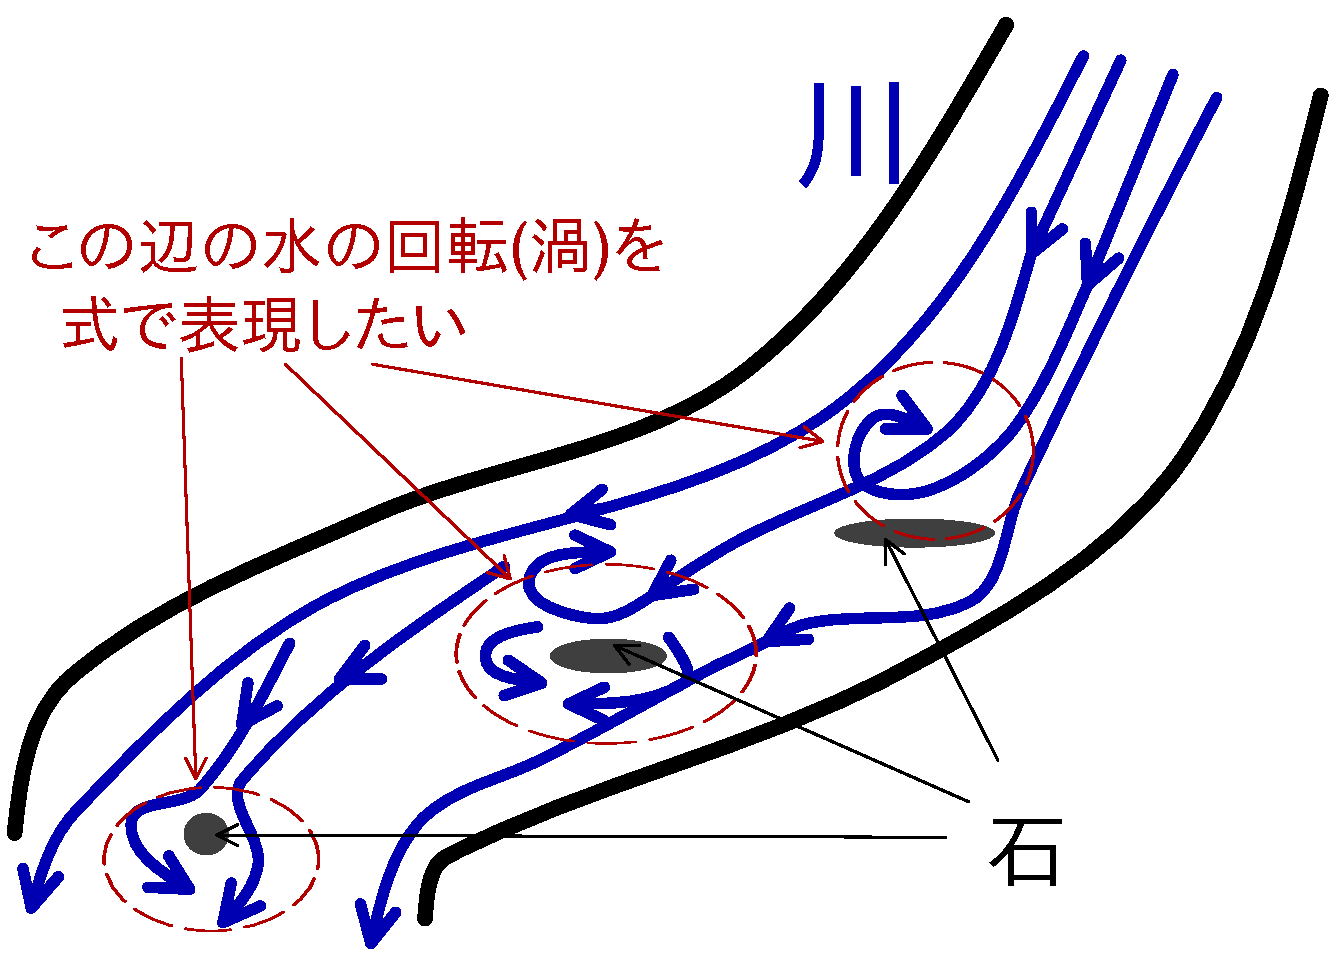
\includegraphics[keepaspectratio, width=4cm,height=2.87cm,clip]{image_rot_1.pdf}
                        \caption{川で生じる渦のイメージ}
                        \label{fig:image_rot_1}
                    \end{center}
                \end{figure}

        物体の回転を扱ったときは,直接的に物体そのものの運動を
        考えることができた.ところが,水などの流体は物体とは異なり,
        その流れ自体を物体と同じように考えるとややこしい.
        そこで,どのような流れかを知るために,川の上に
        葉を置いてみるのだ.葉は,水の流れに従って移動する.
        この葉の動きを観察することにより,
        川の様子を探ることができる.川の全体の
        様子を把握したい場合には,その川のいたるところに
        葉を置いて見て,その葉がどのような動きをするかを,
        観察すればよい.

        葉が1つの場所にとどまっていて,その場で
        回転している状況を想定する.この回転面に $x-y$ 面をとる
            \footnote{
                これは葉が置かれている表面,つまり水面に $x-y$ にとるのと同じである.
            }.
        そして,葉が回転している一点を原点にとる.
                \begin{figure}[hbt]
                    \begin{tabular}{cc}
                        \begin{minipage}{0.5\hsize}
                    \begin{center}
                        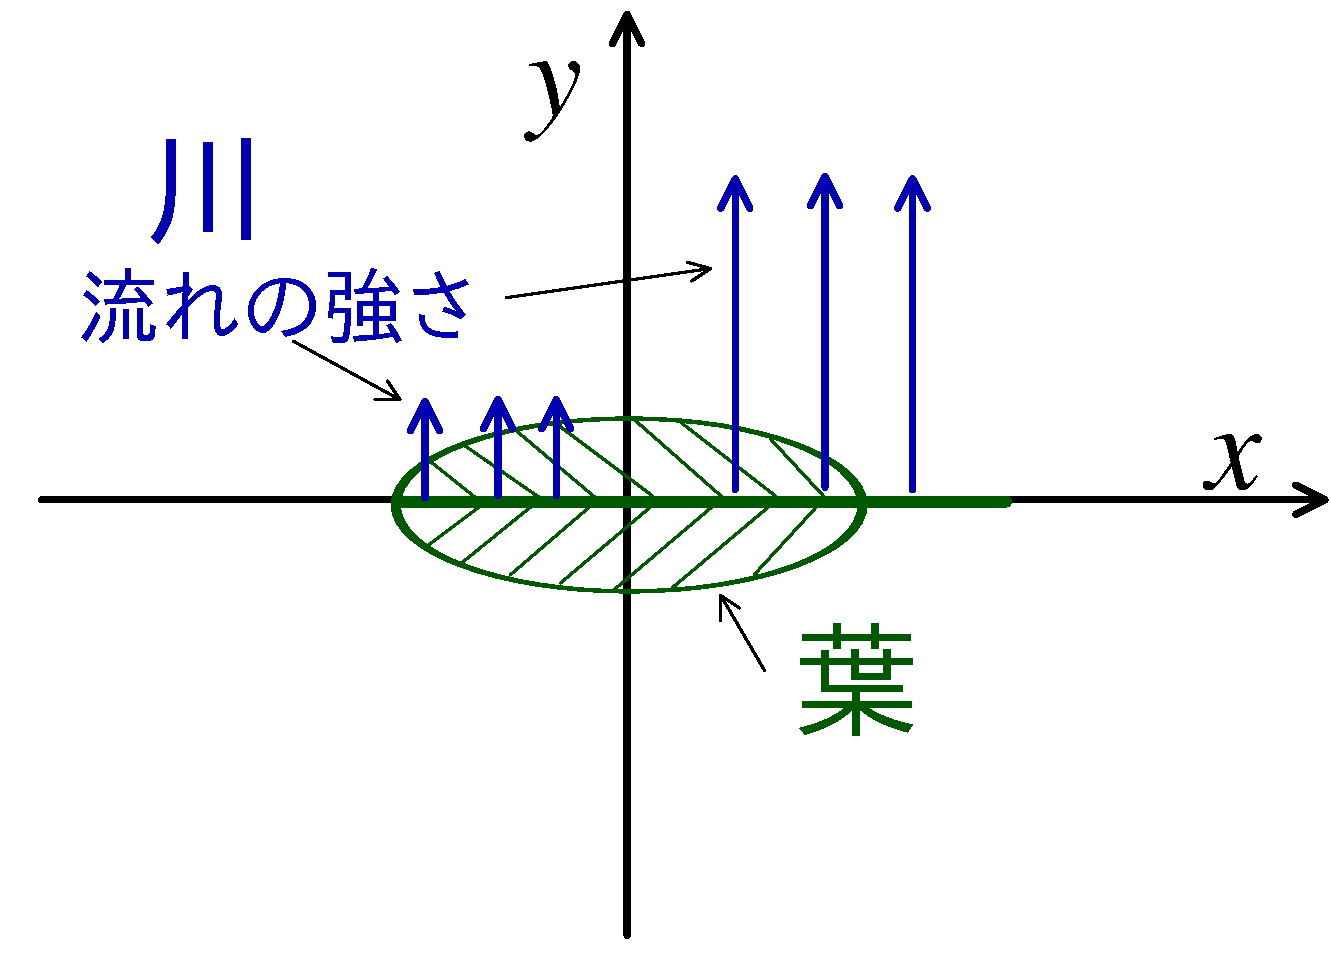
\includegraphics[keepaspectratio, width=4cm,height=2.87cm,clip]{rotrotrot.pdf}
                        \caption{回転(渦)が生じるための条件}
                        \label{fig:rotrotrot}
                    \end{center}
                        \end{minipage}
                        \begin{minipage}{0.5\hsize}
                    \begin{center}
                        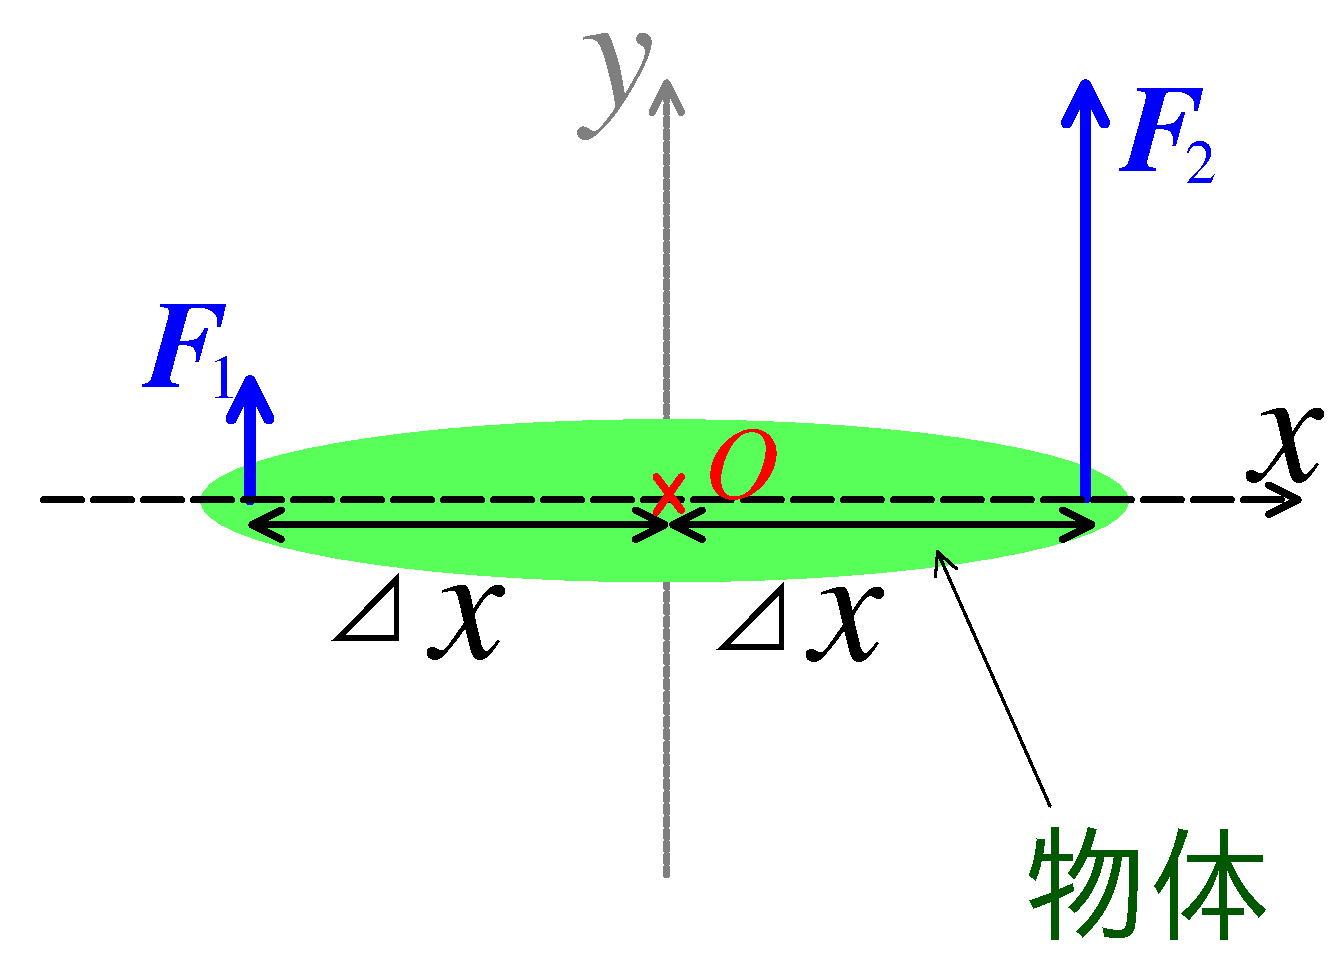
\includegraphics[keepaspectratio, width=4cm,height=2.87cm,clip]{rot_gaiseki1.pdf}
                        \caption{物体(葉)の回転1}
                        \label{fig:rot_gaiseki1}
                    \end{center}
                        \end{minipage}
                    \end{tabular}
                \end{figure}

        葉が原点を中心に回転するには,
        水の流れが原点の中心を境に,
        その勢いが異なっていればよい.
        図\ref{fig:rotrotrot}でいえば,左側の勢いと右側の勢いが
        違っていればよいということである.
        この図はもっと簡単になる.

        この図\ref{fig:rot_gaiseki1}で,左右両方の原点を中心とする力のモーメント
        を考えれば,左側が $F_{1}\Delta x$ であり,右側が $F_{2}\Delta x$ である.
        ここで,図より $F_{1}<F_{2}$ であるから($\Delta x$ は共通であるとする),
        この二つの力のモーメントのは互いに異なった値であり,従って,
        物体は回転をしているはずである
            \footnote{
                回転するように仮定を設けいているので,当たり前と言ってしまえばそうだが,
                確かに回転を表現できるという確認をここでしたのである.
            }.

        ここからが少しヤッカイな部分だが,それは今考えている対象は
        物体の回転ではなく水の回転,つまり“渦”である.
        この渦とはベクトルの回転である.
        物体の回転そのものを
        見るときは力のモーメントを考えればよかったが,
        ベクトルの回転では力のモーメントなんてものは直接には定義できない.
        だから,ベクトル(渦)の上に物体を置いて,その回転でもって
        ベクトルの回転の様子をうかがってみようとしたのである.
        そしてそれによって,ベクトルの回転の様子を,物体の回転として
        観測できることが分かった.この考えをもっと進めていこう.
        簡単のために,原点付近の水の様子を考えてみる.

        力の方向が左右で同じ方向を向いていなくともかまわない.
                \begin{figure}[hbt]
                    \begin{tabular}{cc}
                        \begin{minipage}{0.5\hsize}
                    \begin{center}
                        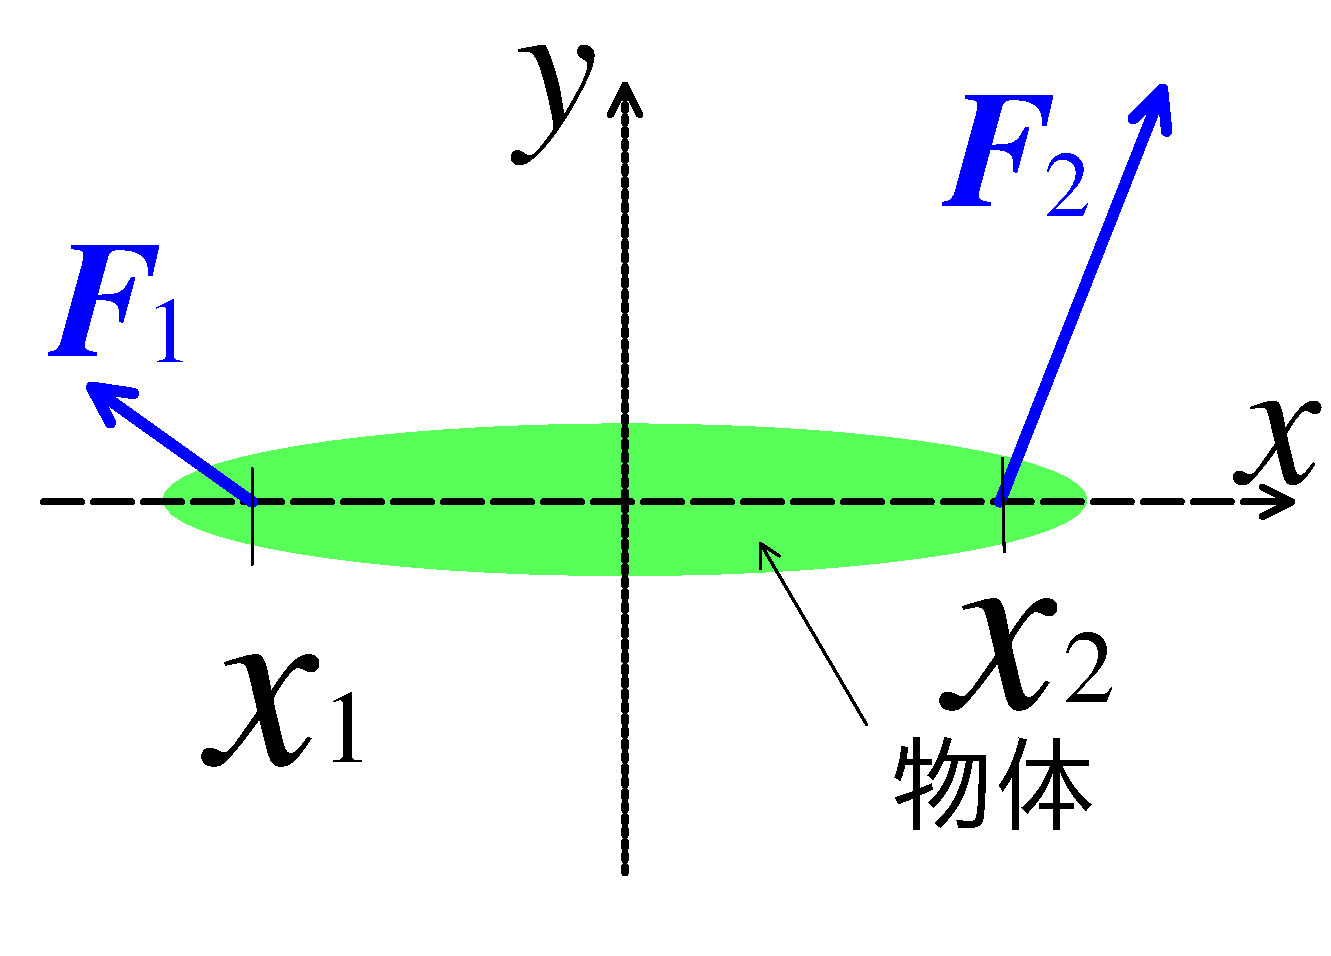
\includegraphics[keepaspectratio, width=4cm,height=2.87cm,clip]{rot_gaiseki2.pdf}
                        \caption{物体(葉)の回転2}
                        \label{fig:rot_gaiseki2}
                    \end{center}
                        \end{minipage}
                        \begin{minipage}{0.5\hsize}
                    \begin{center}
                        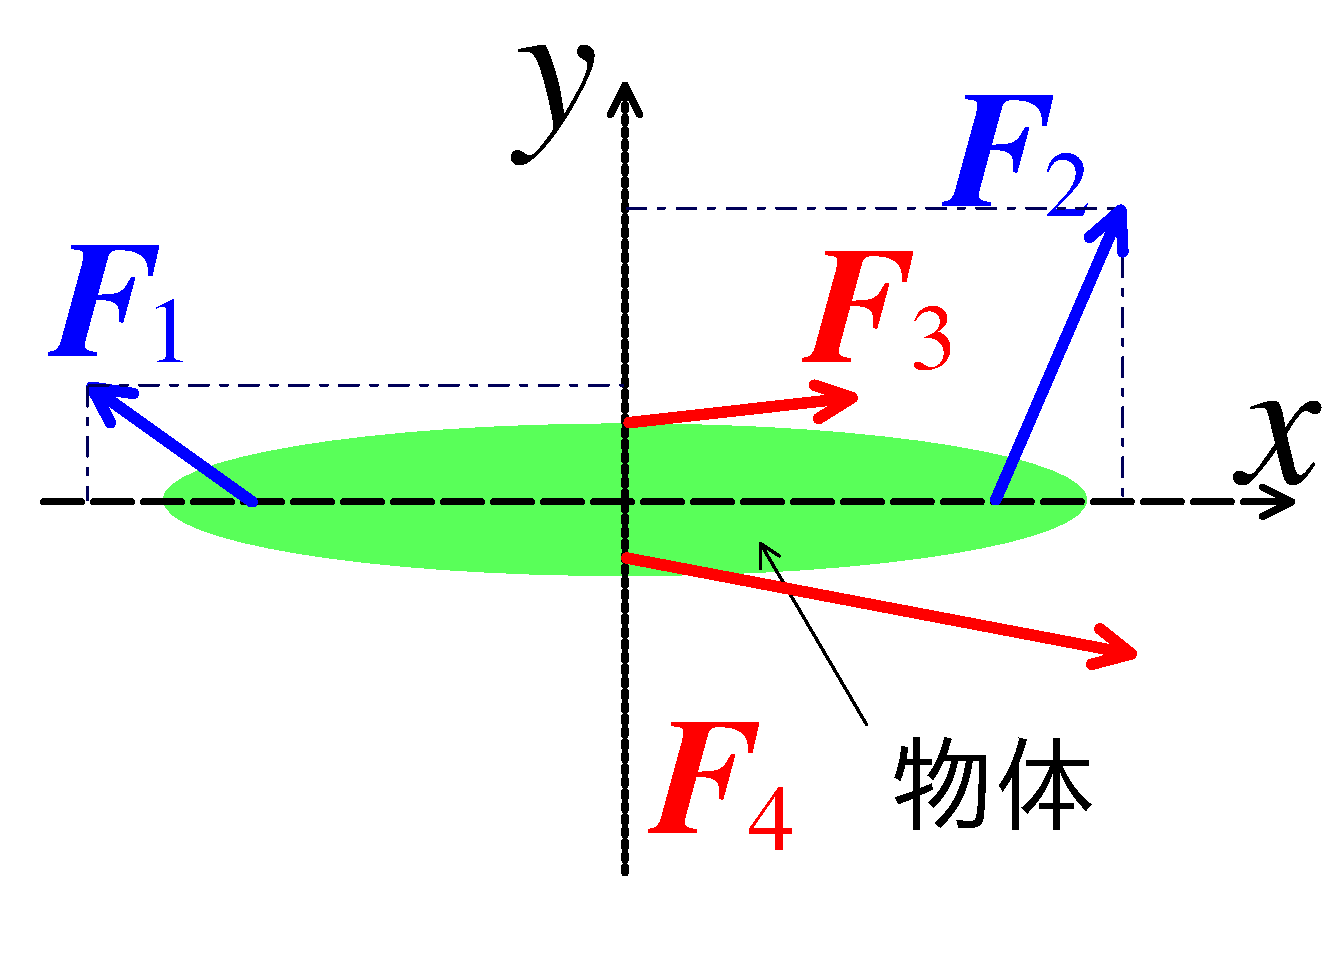
\includegraphics[keepaspectratio, width=4cm,height=2.87cm,clip]{rotation12.pdf}
                        \caption{物体(葉)の回転3}
                        \label{fig:rotation12}
                    \end{center}
                        \end{minipage}
                    \end{tabular}
                \end{figure}

        この図のような状況でベクトルの渦が起こるには,物体にかかる
        $x$ 方向と$y$ 方向の2方向で考えればよい.それを図\ref{fig:rotation12}に示す.

        ベクトル場とはここでは物体が水の流れから受ける力のことだが,
        これを $\bF(\,x,\,y\,)$ とする.
        ここでは話を簡単にするために,ベクトル場は時間に依存しないとした.

        先ほど考えた左右それぞれ力のモーメントの関係は $\bF_{1}\Delta x > \bF_{2}\Delta x$ であった.
        これを以下のように書き直す.
            \begin{align*}
                F_{1}\Delta x - F_{2}\Delta x &>& 0.  \\
                (F_{1} - F_{2})\Delta x &>& 0.
            \end{align*}
        さらにこの式の左辺は0より大きいので,
        何らかの定数,もしくは関数であるので,
        それを $a(\br\,,\,\,t)$ と
        書いて,
            \begin{equation*}
                (\bF_{1} - \bF_{2})\Delta x =a(\br\,,\,\,t)
            \end{equation*}
        とする.今考えている力 $F$ は,$x$ 座標と $y$ 座標ごとに違うはずである.
        つまり,$F$ は $x$ と $y$ の関数であるから,
            \begin{equation*}
                ( F(x_{1} ,\, y_{1}) - F(x_{2} ,\, y_{2}) )\Delta x =a(\br\,,\,\,t).
            \end{equation*}
        今考えているのは,原点付近の水の回転の様子であり,
        $x_{1}$ と $x_{2}$ はさほど離れていないと考えてよい.
        $x_{1}$ と $x_{2}$ の距離は前の図で $2\Delta x$ としていた.
        $2\Delta x$ を $h$ に置き換えてしまおう.
        つまり,$x_{2} = x_{1} + h$ である.
            \begin{equation*}
                ( F(x_{1} ,\, y_{1}) - F(x_{1} + h ,\, y_{2}) )\Delta x =a(\br\,,\,\,t).
            \end{equation*}
        上式の左辺第一項と第二項を入れ替えてみよう.
            \begin{equation*}
                ( F(x_{1} + h ,\, y_{2})  -  F(x_{1} ,\, y_{1})  )\Delta x = -a(\br\,,\,\,t).
            \end{equation*}

        ところで,物体の回転を現すには
        ベクトルの外積を用いた.

        ベクトル $\bA=(A_{x},\, A_{y},\, A_{z})$ の回転 $\drot$ は次式で定義される.
            \begin{align}
                \drot\bA:=
                \left(
                \frac{\rd A_{z}}{\rd y}-\frac{\rd A_{y}}{\rd z}\, ,\,\,
                \frac{\rd A_{x}}{\rd z}-\frac{\rd A_{z}}{\rd x}\, ,\,\,
                \frac{\rd A_{y}}{\rd x}-\frac{\rd A_{x}}{\rd y}
                \right)
            \end{align}

 \subsubsection{ベクトルの勾配($\rm{grad}$)}
        ベクトル $\bA=(A_{x},\, A_{y},\, A_{z})$ の勾配 $\dgrad$ は次式で定義される.
            \begin{align}
                \ddiv\bA:=
                \left(
                \frac{\rd \bA}{\rd x}\, ,\,\,
                \frac{\rd \bA}{\rd y}\, ,\,\,
                \frac{\rd \bA}{\rd z}
                \right)
            \end{align}




 \subsubsection{ベクトル解析の公式(演算子)}
            \begin{align}
                \Delta:=
                \mathrm{div\, grad}=
                \frac{\rd^{2}}{\rd x^{2}}+
                \frac{\rd^{2}}{\rd y^{2}}+
                \frac{\rd^{2}}{\rd z^{2}}
            \end{align}
            \begin{align}
                \mathrm{rot\, rot}
                =\mathrm{grad\, div}-\Delta
            \end{align}



 \subsubsection{ストークスの定理}
        任意の閉曲線を $l$,この閉曲線を縁とする曲面を $S_{l}$ と表す.
        また,閉曲線 $l$ の単位接線ベクトルを $\bt$ と表す.このとき,
        任意の3次元ベクトル $\bA$ に対して,
            \begin{align}
                \int_{S_{l}} (\drot \bA)\cdot\textit{\textbf{n}}\,\df S_{l}
                =\oint_{l} \bA\cdot\bt\,\df l
            \end{align}
        が成り立つ.これを \textbf{ストークスの定理} という.



\chapter{行列}
%   %-----------------------------------------------------------------------------------------------
%   %  Input
%   %    File Name : PhysNote_Math_Matrix.tex
%   %    説明      : 「行列」について.考え方と使い方.
%   %-----------------------------------------------------------------------------------------------
        %===================================================================================================
%  Chapter : 行列
%  説明    : 行列の基本的な計算規則,座標変換について
%===================================================================================================
%   %==========================================================================
%   %  Section
%   %==========================================================================
    \section{行列とは}



%====================================================================================================
%  以降は,付録(Appendix)
%====================================================================================================
    \appendix

%===================================================================================================
%  Part : 思想
%  説明 : 思考の基礎・基本を考える
%===================================================================================================
    \part{思想}
%   %-----------------------------------------------------------------------------------------------
%   %  Input
%   %    File Name : PhysNote_Introduction.tex
%   %    説明      : 「思想」トップファイル
%   %                表現(言語,絵),知覚・直感・思考 等 について,考える
%   %-----------------------------------------------------------------------------------------------
        %===================================================================================================
%  Chapter : 感覚・思想・表現
%  説明    : 物事を考える上での,根本的な思想を記述する
%===================================================================================================
\chapter{感覚$\cdot$思考$\cdot$表現}
    \begin{mycomment}
        この章は,私の個人的な考えをメモしておくものである.だから,記述内容が
        誤っているかもしれず,考え違いや,誤解が含まれていることと思う.
        誰とも議論もせずに記述することであるから,偏った考え方になりがちだし,
        最悪の場合,矛盾がふくまれているだろう.それにもかかわらず,
        この章の文章は"言い切り"の形で記述する.いちいち,「だと思う」という
        語彙を文章末尾につけてしまうと,読みにくくなってしまうし,第一,カッコ悪い.
        なので,偏った考え方や誤った主張を強く強調していると思われるかもしれないが,
        そうではなく,単に現在の私の考えをメモしているものに過ぎないと,捉えてもらいたい.
    \end{mycomment}
%   %==========================================================================
%   %  Section
%   %==========================================================================
        \section{根拠なしに,確信できること}
            根拠なしに確信を持てることは,「考えられる」ということである.
            そして,考えるという行為は,言葉
                \footnote{
                    ここで言う \textbf{言葉} とは,“書くことによる表現”と“話すことによる表現”
                    の両方を指す意味で使っている.
                }
            を用いて行われてることも,根拠なしに
            認めることができる
                \footnote{
                    「言葉なしに考える」という行為は可能だろうか.
                    少なくとも,私には実行不可能である.
                }.

            何かものを考えるときには,考えるための材料と道具が必要である.
            材料というのは経験であり,道具というのは言葉である.
            考えるという行為とは,経験を道具により整理して,その経験に対する
            理解を深めるという行為である.

            私たちの経験する全ての事柄を,\textbf{世界} と表現することにしよう
                \footnote{
                    ここでいう \textbf{世界} とは,世界の国々を表しているのではない.
                    私たちが目や耳などの,いわゆる五感で感じ取る全てのことを総合して,
                    「世界」と表現する.
                }.
            私たちは,世界を経験をできる.経験を記憶できる.
            また,経験を不思議がったり,その不思議を考えられる.
            そして,その考えを言葉や絵で表現できる.そして,このような表現を
            行うことで,自分以外の相手に自分の考えを伝えることができる.

            これが,私の「考えること」の根本的な思想である.これからの物理学の学習は,
            この思想のもとに行う.

            \begin{memo}{言葉と思考の順序}
                考えるという行為は,言葉を使って行われう行為である.もっと強い言い方を
                すると,考えるという行為は言葉なしに行うことは不可能である.つまり,
                言葉を習得する以前は,ものを考えることができないことになる.
                となると,言葉の見習得の赤ん坊は,ものを考えることができないのだろうか.
                この問題に対する,私が納得のできる答えは,まだ存在していない.

                しかし,これだけは言える.言葉の習得する以前から,この世界を感じている.
                世界を感じるという経験の1つに,言葉がある.経験が「思考する」という
                行為の基礎に位置するのである.しかし,この推論に確証はもてない.
                経験が思考の基礎をなすということ
                を,今から身をもって体験することができないからだ.
                言葉習得以前の状態にもどり,言語を習得しなくとも世界を感じとることが
                できるのだな,という感覚を体験できればよいが,これは不可能である.
                推論をいくら重ねたところで,あるいは,多くの言語見習得の赤ん坊を
                観察したところで,自分自身で実感できないので,納得はできない.
                納得はいかないけれど,今の私は言語を扱っている
                    \footnote{
                        少なくとも,とりあえずの不都合なく,意思疎通ができる程度に.
                   }.
                また,その習得に多くの時間を費やしたことも記憶にある.ということは,
                言語見習得の時期があったいう推論は妥当であるとも思える
                    \footnote{
                        実際に言語見習得の時期の記憶がないので,単なる推論でしかない.
                    }.
            \end{memo}

            \begin{memo}{言葉の習得}
                言葉は,人間が生まれながらにしてもっているものではない.
                言葉は,意思疎通を行うために,先人の経験により発明され,
                洗練されてきたものである.

                私たちは,生まれてから自然と母国語の文法を習得する
                    \footnote{
                        国語の時間に,強制的に習得させられることもあるだろう.
                        ひらがなや,カタカナ,漢字を覚えるのには苦労したはず.
                        また,使い慣れない語彙を使用し始める場合,単語そのものを
                        誤って使ってしまい(「つくる」を「くつる」に間違うなど),
                        大人から,その場で間違いを指摘され,修正された経験もあったことだろう.
                        しかし,その間違いの指摘は言葉によって行われたのであり,
                        それにより,誤りを自覚してそれを修正しようと努力できたはずである,
                        全ての言葉を自然に習得できるわけではないのだが,言葉の基本的な使い方
                        は誰から教わったものではなく,自分の周囲に飛び交っていた母国語を
                        聞くことにより,非言語的に習得するのである(
                        そうでなければ,言葉の使い方を間違っときの,その間違いの指摘を
                        理解することができないことになる).
                        言葉の文法を,0から
                        言葉により説明することはできない.というのも,文法を説明しようとすると,
                        その説明自体に言葉を使用せざるを得ず,
                        つまり,「文法を知る前に文法を知っていなければならない」といった,
                        自己言及的な矛盾がおこるからである.しかし,現に私たちは母国語の文法を
                        習得して使用している.
                    }.
                母国語は体系的に教わることない.常に生の言葉を聞き,そして,その時の状況を
                機能するすべての感覚器から感じ取り,言葉の使用法を身につける.論理学や数学
                で言うところの公理
                    \footnote{
                        最も基礎となる,疑いようのない事実のこと.万人が根拠なしに正しいと
                        感じること.例えば,数学で言うと,「A$=$B で B$=$C のとき,A$=$C」
                        といった感じの,最も基本的なお約束のことを言う.これは有無を言わさず
                        たたきつけられることである.その根拠を求めてはならない.公理の根拠
                        なんてものは,はじめから存在しないのだから.言い方を変えれば,何かを
                        論理的に考えようとした時に,その根拠が求められることがあるが,
                        その根拠は果てしなく問うことは不可能である.いずれは,根拠を示すことができない
                        当たり前すぎる事柄に,直面することだろう.それを公理というのである.
                    }
                があるわけでもなく,ただ漠然と,その使われ方を悟り,自分のものとしていく.
                人間には,言葉を習得する能力が生まれながらにして備わっているのだ.
                なぜだろうか.意思疎通をうまい具合に行うためだとか,いろいろ後付的な
                説明がなされることもあろうが,そんなことは確かめようがない.なんとでも言えるのだ.
                ここでは,深く考えずに,「私は言葉を使うことができる」ということを,
                素直にそのままの形で受け入れておこう.
            \end{memo}

            \begin{memo}{意思疎通}
                言葉はどんな時に使われるのだろうか.いや,おかしな疑問を投げかけてしまった.
                そんなの,意思疎通を行うために決まっているじゃないか.本当に,そうなのか.
                言葉でだけで,意思疎通が十分に可能だろうか.いや,できないはずだ.
                誤解や言い間違いなどで,正しく意思疎通ができないこともあるだろう.
                言葉だけで十分に意思疎通はできないのは,当たり前で,そのために,他の手段として,
                手や体を動かして(身振り手振り)表現することもある
                    \footnote{
                        別れ際に相手に対して手を振ったり,違うことを示すために首を横に振ったりするだろう.
                    }.
                図を使って表現することもあろう.音楽で気分を表現したりもするだろう
                    \footnote{
                        気分が良い時には,鼻歌が自然にでたり,踊ることだってするでしょ?
                    }.
                とにかく,意思疎通のための道具は,言葉だけではない.

                だけど,ここまで書いといてなんだけども,ノートで自分の考えを示すのには,
                図と言葉でしか表現できない.なんともやりづらいが,どうしようもない.
                ここは我慢して,図と言葉だけで伝わるように,記述しなければならない.
                図と言葉だけで,どれだけのことが表現できるかわからないが,頑張って考えながら,
                記述していこう.たとえ時間がかかろうとも,文が長ったらしくなろうとも,
                丁寧に記述していけば,どんなことでも言葉で伝えることができると信じて,
                記述していこう.

                私は考えることができ,それを言葉で表現でき,そして,
                その言葉によって他者に自分の考えを伝える事ができると信じる.
                そして,逆に,他人の表現する言葉を理解し,他者の考えを受け入れられることも,信じる.
                さらに,自分と他人とで会話を続けることにより,より深く正確に互いの考えを
                理解し合えると信じよう.ここのところをこれ以上疑いだすと,言語哲学的な世界に
                陥ることになり,抜け出せなくなってしまう.もうこれ以上,言葉について考える
                事はせずに,話を先に進めよう.
            \end{memo}

%   %==========================================================================
%   %  Section
%   %==========================================================================
        \section{表現}
            思考を表現する最も有効な道具が,言葉である.また,時には,言葉よりも絵に書いたほうが
            より伝わりやすいこともあろう
                \footnote{
                    宣伝看板や,ポスターなどが良い例だ.
                }.
            言葉や絵以外にも,ある規則に従った記号により,思考を
            表現することも可能である.
                \footnote{
                    特に,音楽は言葉によって表すことは難しい.原理的に不可能とは言わないが,
                    そうして表現できたものは,とても煩雑で理解しがたい表現になっていることだろう.
                    では,音楽を伝える方法はないのかというと,もちろん,そんなことはない.
                    周知の通り,\textbf{楽譜} という音楽独特の表現方法が考えだされている.
                    楽譜は絵でも言葉でもないが,人間のもっている,ある種の感覚を表現するものである.

                    また,他例を上げれば,数学や記号論理学なども,記号の羅列である.

                    「言葉」という語彙は,これらの例のような意味を含めて使われることも多い.
                    これは,文脈によって理解できるだろう(著者はそうわかるように書くべきだ).
                }.
            表現するという行為は,言うまでもなく,
            自分の考えや思いを自分以外の相手に伝えるということである.

%   %==========================================================================
%   %  Section
%   %==========================================================================
        \section{「科学」の思想}
            "科学的" という言葉は日常的に使用される.特に,最新技術という意味で
            使用されることが多いように感じる.しかし,"科学的" とはどういうことかを
            考えてみると,残念なことに,明確なイメージを描けないことに気付く.

            \begin{figure}[hbt]
                \begin{center}
                    \includegraphicslarge{SekaiKansokuBunrui01.pdf}
                    \caption{科学的に扱えることの範囲}
                    \label{fig:ThomomExpElec001}
                \end{center}
            \end{figure}

        \begin{memo}{基礎がない,考えが循環する}
            ものごとを考える前には,経験が必要である.考えは,その経験の不思議さ
            を基に行われるからである.では,この経験はどう捉えら得るのだろうか.
            当然ながら,経験は眼や耳などの五感で捉えられる.そして,その認識は,
            脳に伝わって初めて経験を実感し,記憶される.だから,最も基礎的な
            学問分野は脳科学なのだろうか.いや,これは違う.脳は生物の一部であり,
            脳科学は生物学の一分野として位置するものである.生物はその組織の
            内部で,化学反応を起こして生命を維持している.従って,化学が,生物学よりも
            基礎的な位置にあるはずである.また,化学で扱われる化学反応は,突き詰めれば,
            原子や分子の結びつきであり,原子や分子の運動は物理学により説明される.
            そして,物理学は数理的推論をその拠り所としていて,数学と論理学が物理学
            の基礎となっている.数学と論理学は,元を正せば,私達が日常生活の中で使用している
            言語の曖昧な部分を除き,正しい思考とは何かを探る学問である.そして,その思考を
            行うには,前もってその思考に関する経験が必要である.経験は五感で感じ,脳によって
            認識され,$\cdots$.

            循環する.上記のどこかに誤りがあるのだろうか.
        \end{memo}

%===================================================================================================
%  Chapter :
%  説明    :
%===================================================================================================
\chapter{論理}


%===================================================================================================
%  Part : 思うこと,思ったこと
%  説明 : 自分なりの考え方・思想についての記述を行う.
%===================================================================================================
    \part{思うこと,思ったこと}
%   %-----------------------------------------------------------------------------------------------
%   %  Input
%   %    File Name : PhysNote_Omoukoto.tex
%   %    説明      : 物理学を考える以前の,基本思想を記述する.
%   %-----------------------------------------------------------------------------------------------
        \normalsize
%%**************************************************************************************************
%%
%% File Name : PhysNote_MessageFirst.tex
%% 説明      : 物理学の導入をかねた,古典力学(ニュートン力学と解析力学)を学習する.
%%
%%**************************************************************************************************

%===================================================================================================
%  Chapter : 素朴な疑問
%  説明    : 「考えるとはどういうことか」とかを考えてみる.
%===================================================================================================
    \chapter{素朴な疑問}
%   %-----------------------------------------------------------------------------------------------
%   %  Input
%   %    File Name : PhysNote_Math_MsgFirst.tex
%   %    説明      : 考えるって何だろう.
%   %-----------------------------------------------------------------------------------------------
        %===================================================================================================
%  Chapter : はじめに
%  説明    : 「考えるとはどういうことか」とかを考えてみる.
%===================================================================================================
%   %==========================================================================
%   %  Section
%   %==========================================================================
        \section{最も基本的なこと}
            学問を学ぶにあたって,“最も基本的で信頼できること”を
            基礎にして,その上で学習を進めることは,当たり前のこと
            である.では,その“最も基本的で信頼できること”とは何
            だろうか.

            これは多分に哲学的な問題提起であるが,ここでは,今後,
            物理学の学習を進めていくにあたり,思想の最も基本的なよ
            りどころを確認するためのもので,哲学に深く介入すること
            はしない
                \footnote{
                    正直に書こう.哲学に介入することは,私のような
                    低レベルの頭では,不可能である.開き直って,言
                    うならば,そこまで深く考えてもしょうがない,思
                    うところもある.
                }.

            私は,最も基本的で信頼できることとして,「考えること」
            をあげたい.これは独我論てきな思想である.独我論とは,
            極端に言えば,この世界に存在を確信できるのは私の思考の
            みであり,私が今感じている温度や光などは,私の思考によ
            って感じていると錯覚しているのであって,実在しているの
            ではない,という考え方である.こう考えると,自分以外の
            人間とは,私の思考が作り出した幻想であり,実際にそこに
            いるわけではないということになる.そう,信じられるのは,
            今考えている私がここにあるということである.


%   %==========================================================================
%   %  Section
%   %==========================================================================
        \section{私の思想の根本}
            では,もう一段階突っ込んでみよう.「考える」ということ
            とは,どうすることなのだろうか.「考える」という動詞の
            使い方は,おおよそ次の様だろう.
                今晩の献立を考える.
                人の気持ちを考える.
                将来の進路を考える…
            などなど.
            考えるという作業を行っているとき,「言葉」を道具として
            使う.また,時には「図」を使って考えることもあるだろう
            が,これは単に言葉で考えるよりも図を用いた方が考えやす
            いからであり,言葉では思考不可能であるということではな
            い.思考はすべて言葉で表現できる(と信じる).

            私の,最も信頼できる唯一の基本的なことである,私の思考
            は言葉を用いて実行される.では,その次の疑問として,
            「言葉」とは何か,ということが生まれてこよう.

            この章では,「考えるとは何か」について,私が考えること,
            というか,思っていることを記述する.


%   %==========================================================================
%   %  Section
%   %==========================================================================
        \section{思考の道具}
            考えるという動作は,言葉を用いて行っていることを確認し
            た.言葉を用いて考えているので,この言葉の使用限界が思
            考の限界であるということになる
                \footnote{
                    Wittgensteinは「論理哲学論考」という著
                    作で,このことを詳しく論じている.後に,彼自身
                    によってこの著作は間違いであるとされてしまうの
                    であるが…このノートでは,そこまで深く入ら
                    ない.だって,とっても難しいから.
                }.

            単に「言葉」といっても,それは様々な形で存在する.英語
            やドイツ語,フランス語,イタリア語などたくさんだ.各国
            の人々は,自国のあるいは使い慣れた言葉で考えていること
            だろう.ここでは,どのような国の言葉も,その適用限界
            は変わらないと仮定して,話を進めて生きたい.多少,言葉
            の適用限界があったとしても,それは話にならないくらい,
            細かいことに過ぎないと信じる
                \footnote{
                    実際,各国の人々が同じように「考えて」いるとい
                    う現状からこのような仮定を設けてもよいと考えて
                    いる.ただし,ここでは,「考える」ということに
                    関して,文化や伝統,生活習慣などの影響は無視す
                    る.
                }.

             もちろん,言葉で説明できないこともある.ある種の“ひらめき”
             とか,もろもろの感情とかを言葉で表現することは難しいこ
             とである.いや,不可能といってもよい.しかし,考えると
             いうことに関しては,言葉のもつ機能は十分である考える.私
             は,「どんな思考も言葉にできる」と信じて,こ
             のノートを作成する.


%   %==========================================================================
%   %  Section
%   %==========================================================================
        \section{言語の曖昧さ}
            思考を言葉で記述できたとしよう.その次に問題となるのは,どれ
            だけ正確に思考できるか,ということだろう.いや,視点を変えて
            言い換えよう.私たちが行う多くの思考の中で,正しい思考とはど
            ういうものなのかを,整理しなければいけない.わけのわからない
            思考や,意味を成さない思考などを排除したいのである.


%   %==========================================================================
%   %  Section
%   %==========================================================================
        \section{日常言語}
            普段の生活で使っている言語は,曖昧な表現をすることが多い.曖昧
            表現というのは,人によって解釈が異なってしまう表現のことである.
            「美しい景色」だの,「大きな木」だのと言って,すべての人が同じ
            情景を浮かべることはまずない.これでは正しい思考が,十分ではな
            い他の人間に伝わることはない.

            しかし,このような例から,普段使っている言語は正しい思考に適し
            ていないと,判断してはいけない.事実,過去の多くの頭のいい学者
            さん達は,言語を用いて正しい思考をし,様々な学問を作り上げてい
            る.大切なのは,曖昧な表現を避けることである.ただ,言語には使
            い方によって,曖昧に表現できてしまうだけなのである.

            では,言語の曖昧な表現を使わないようにするには,どうしたらよい
            だろうか.まず考えつくのは,日常言語から万人が認める最も基本的
            な部分を抽出し,それを元に思考をすればよいことである.言語の最
            も基本的な部分とは,「論理」である.次に,論理について簡単に触
            れよう.




%===================================================================================================
%  Chapter : 論理学とか,数学とか
%  説明    : 物理学より,思考方法としてより基礎的なことである,論理・数学について考えてみる.
%===================================================================================================
    \chapter{論理学とか,数学とか}
%   %-----------------------------------------------------------------------------------------------
%   %  Input
%   %    File Name : PhysNote_CM_LogicMathEtc.tex
%   %    説明      : 数学とか論理学について,物理学のもっと基礎にある学問についての断片的な学習メモ.
%   %-----------------------------------------------------------------------------------------------
        %===================================================================================================
%  Chapter : 論理学とか,数学とか
%  説明    : 物理学より,思考方法としてより基礎的なことである,論理・数学について考えてみる.
%===================================================================================================

%   %==========================================================================
%   %  Section
%   %==========================================================================
        \section{論理}
            私たちが普段の生活で使っている言語のうち,曖昧な使い方を避けて
            ,万人に共通に伝わるようにしたい.そのためには,\textbf{論理}
            と言うものを考える必要がある.論理は,日常言語の中の一部にある
            .相手に自分の考えを伝えるとき,物事を筋道立てて伝えようとする
            だろう.自分の考えをできるだけ性格に相手に知ってほしいからであ
            る.さて,このとき私たちは,論理を使っているのである.論理は,
            何個かの公理
                \footnote{
                    公理:万人が認める事実のこと.何の反論なしに認めなけれ
                    ばならないことである.ある仮説を検証するとき,その仮説
                    の根拠をどんどん探ることになる --- AはBとCからなってい
                    て,BはDから,CはEを基にしている・・・と言うように---.
                    しかし,いつまでもこれが続くわけではない.いつかは,ど
                    うしようもなく“当たり前すぎて”,説明ができないことに
                    たどり着く.公理とは,その当たり前の事実を明示するもの
                    である.
                }
            と推論規則
                \footnote{
                    推論規則:ある仮定から,別の仮説を作り出せる規則のこと
                    .公理と同様,有無を言わさず認めさせられるものである.
                }
            を基に構成される.少数の公理と推論規則から,主張したいことがす
            べて主張できる体系を作ることが学問の目的である.これを思考経済
            と言ったりする.公理と推論規則は,少なければ少ないほどよい.



%   %==========================================================================
%   %  Section
%   %==========================================================================
        \section{論理学}
            この論理について,詳しく研究する学問に \textbf{論理学} がある
            .ある仮説を記述した文で,本当か嘘かをはっきりと区別できる文の
            ことを,\textbf{命題} という.論理学はいくつかの必要最小限の公
            理と推論規則を組み合わせ,命題の証明を繰り返し発展させていくも
            のである.命題と推論規則の組み合わせのことを,\textbf{公理系} と
            言う.この公理系には,次の3つの性質が備わっている必要がある.一
            つは \textbf{独立性} で,公理形の中のどの1つの公理を選んでも,
            他の公理からその公理を証明できないような性質である.
            二つ目は \textbf{完全性} と言われるもので,主張したい命題が,そ
            の公理系からすべて導けることである.三つ目は \textbf{無矛盾性} と
            言われるもので,公理系に互いに矛盾する公理を含んでいないことで
            ある.

            論理学とは考察の足固めである公理系を設計し,体系を作り上げて
            いく学問でもあるのだ.どれだけ詳しく説明できるかと言う疑問の最
            も根本的な部分の研究がここでなされる.



%   %==========================================================================
%   %  Section
%   %==========================================================================
        \section{数学}
            数学とは,論理に複素数を組み合わせた学問であると言える.その研究
            の対象はおもに,複素数である.複素数の一部には,自然数が含まれて
            いる.残念なことに,自然数を含む公理系には,完全性,無矛盾性が常
            に保たれていると言う保障がないことが知られている.この事実は
            G\"{o}delの \textbf{不完全性定理} とよばれている
                \footnote{
                    参考文献:廣瀬 健,横田 一正 [著],「ゲーデルの世界」,
                    鳴海社,2004
                }.

            集合論により無限を扱えるようになってきたころ,この無限を起因とし
            て様々なパラドクスが発見されることとなった.「自分自身を要素とし
            て含まないすべての集合」がその最も有名なものである.ちょっと考え
            てみよう.
                \begin{equation*}
                    \omega:\;\;\mbox{自分自身を要素として含まないすべての集合}
                \end{equation*}
            と定義しよう.そして,次の問題,すなわち
                \begin{equation*}
                    \mbox{問題}:\;\;\omega \mbox{自身は,} \omega \mbox{に含まれるか否か}
                \end{equation*}
            を考えてみよう.すぐに明らかな矛盾が見えてくるだろう.

            $\omega$ は自分自身に含まれると仮定してみる.すると,$\omega$ の
            定義「自分自身を要素として含まない」という仮定に矛盾する.では,
            $\omega$ は自分自身に含まれないと仮定したらどうか.実はこれでも
            矛盾が生じる.なぜなら,「自分自身要素としてを含まない」という
            定義上,仮定で「自分自身は含まない」言っているので,自分自身を
            含むべきだと言う結論が出てしまう.肯定的に仮定しようが,否
            定的に仮定しようが,どちらにしても結果はその仮定と矛盾するので
            ある.

            Russellらは,この問題を解決しようと階という概念を導入し,命題
            に自分自身を含むことのないように制限を加えた.しかし,問題はこれ
            だけではとどまらず,山のように残されていた.

            Hilbertはこのような問題の山を,数学の危機であると自覚し,これを
            解決しようと計画した.Hilbertはこの数学の危機と言われる問題を23
            個の命題にまとめた.そして彼は,この23の問題を証明し解決しようと
            呼びかけた.G\"{o}delの不完全性定理はこの23の問題のうちの一つ
                \footnote{
                    第2番目に掲げられていた問題だった.
                }
            の否定的な回答であった.

            だから,物理学に公理系を作成して,論理的に構成しようとしても,無駄
            である.しかし,物理学は自然の構成を探る学問だから,この点に関して
            はあまり気にすることはないと思う.


%   %==========================================================================
%   %  Section
%   %==========================================================================
        \section{物理学}
            物理学は,自然がどのようになっているかを探る学問である.
                \footnote{
                    "なぜ"自然が私たちの感じているようになっているのかを探る学
                    問では\textbf{ない}.
                }
            「なぜ(Why)」を問うのではなく,「どのように(How)」を問うのであ
            る.

            なぜ自然がこのように
                \footnote{
                    普段の生活で,私たちが感じている自然を思い浮かべてみて.
                }
            なっているのか,とか,なぜ宇宙があるのかとかを考えるのは哲学であって,
            物理学ではない.物理学ではこういう,"なぜ"を問うような疑問には答えられない
                \footnote{
                    ただ,"なぜ"という問を深めていく事は可能で,実際に,物理学の発展は
                    その繰り返しである.その様子は.これからの学習で実際に感じることになる.
                }.

            物理学とは,自然の性質を見つけるものである.この「性質」という言葉は
            物理学では \textbf{法則} と呼ばれている
                \footnote{
                    \textbf{法則}:後で詳しく記述する.
                }.
            自然の法則を,実験や数式を通して見つけ出すことが物理学の目的なのだ.

            自然はデタラメに変化しているのではなく,何か一定の法則に従ってい
            るということは,経験上理解できることと思う.例えば,特別に力を加え
            ない限り,高いところから低いところへ,物体は落ちていく.落とした消し
            ゴムは,拾わないと手元に戻ってこないのである.何でだろうか.この原因
            を探り,「法則」として記述するのである.

            このことについては,物理学を学び始めた段階ではまだ実感がわかないかも
            知れない.学習していく過程で,だんだんとわかることだろう.

            このノートでは物理学を学習することが目的である.自然はどのような法則
            に従って変化しているのだろうか.少しずつ考えることにしよう.




%===================================================================================================
%  Chapter : 他愛のない,思ったこと
%  説明    : 他愛のない,思ったことをメモしおこう.
%===================================================================================================
    \chapter{他愛のない,思ったこと}
%   %-----------------------------------------------------------------------------------------------
%   %  Input
%   %    File Name : PhysNote_Apdx_Omoukoto_TaaiNaiOmoukoto.tex
%   %    説明      : 
%   %-----------------------------------------------------------------------------------------------
        %===================================================================================================
%  Chapter : 他愛のない,思ったこと
%  説明    : 
%===================================================================================================

%   %==========================================================================
%   %  Section
%   %==========================================================================
        \section{生まれ変わる?}
            「生まれ変われるとしたら,次は何になっていたい?」と聞かれることが
            ある.この質問には,何も考えずに答えることが,コミュニケーションを
            円滑にする為に良いのだが,やはり引っかかる部分がある.

            引っかかることとは,「生まれ変わる」ということの定義である.生まれ
            変われるか否かということも当然疑問なのだが,それよりももっと疑問な
            ことがある.生まれ変われることが可能かどうかという疑問には,おそら
            く答えることは不可能だろう.生まれ変わることが不可能であるとした
            ら,話はそれで終わりであるので,ここでは,生まれ変われることができ
            るものとして,話を進めたいと思う.

            疑問というのは,“今の記憶が忘れ去られていたとしても,生まれ変わったと言えるか”と
            いうものである.以前までの記憶がない以上,当然,自分自身には生まれ変わ
            ったという意識は生まれない.第三者的な立場にたって,他人の生まれ変
            わる瞬間を見たとしよう.その場合,生まれ変わることが可能だと,納得
            することだろう.しかし,その他人には以前までの記憶がなく,やはり,
            その人にとって,生まれ変わったという意識はないはずである.たとえ,その瞬間を見てい
            たと教えてやったとしても,その人は生まれ変わったのだと明確に認識することは不可能である.

            生まれ変わって以前までの記憶がない以上,たとえ本当に生まれ変わったのだとしても,
            自分自身にとっては,別人であると意識せざるを得ないと考えるのが,自然なのではなかろうか.
            実際,今の私には,こう考えることが一番妥当だと思っている.
            たとえ,生まれれ変わっていたとしても,記憶が残っていない以上,
            それはその人にとって別ものなのだと考えたい.

            まとめよう.求める答えは,生まれ変われるか否か,ということだったが,これには,
            答えることはできない.
            生まれ変わることができないのであれば,話はここで終了になる.もし,
            生まれ変われることがわかったとしても(他人が生まれ変わったことを見るなどして),
            自分自身では認識できないのであれば,それは生まれ変わったと考えるべきではない,
            と思う.

%   %==========================================================================
%   %  Section
%   %==========================================================================
        \section{教科書に書かれていること}
            物理学や化学$\cdot$生物学$\cdot$天文学などの自然現象を説明すべく,それを
            文字として記述し,本という形で記録できる.
            世の中には多くの専門書,教科書,解説書がある.しかし,
            どれをとっても自然現象をすべて説明するものはない.
            つまり,本を読んだところで,世界を理解できるわけではない.
            本を読んでわかることは,先人たちが苦心して築きあげてきた
            壮大な理論体系ではあるものの,自然現象についてのほんの僅かな
            ことでしかない.

            物理学を学ぶということは,物理学の論文や専門書,教科書を
            読むということではなく,実際の自然現象に触れるということ
            である.そして,なぜだろうと疑問に感じることであり,
            さらに,それを解き明かしたいと思うことである.

            物理学を学びたいから物理学の教科書を読む,なんてことは,
            甚だ見当違いである.物理学は自然現象を説明する理論であり,
            つまり,実際に起こっている現象を説明しようとするものである.
            重要なのは,現象に触れること.そして,その現象について,
            その特徴をできるかぎり詳しくしらべること.そうしてやっと,
            現象の特徴はどのような法則に従っているかといった,理論的
            研究に入るのである.

            物理学の本を読むということは,今知られている理論を把握
            するということであり,物理を追求するという行為ではない.
            あくまでも,先人の得た知恵を吸収するということである.
            しかし,それは,探求の第一歩ではない.
            物理学の本を読んで,物理をわかった気になっているとしたら,
            とても残念なことである.


%   %==========================================================================
%   %  Section
%   %==========================================================================
        \section{心配レベル}
            心配という心情には,4つの段階があると思う.それは,次の通りだ.
                \begin{enumerate}
                    \item 心配
                    \item 不安
                    \item 恐怖
                    \item 絶望
                \end{enumerate}
            下に行くほど(数字が大きくなるほど),心配レベルが上がる.
            
            具体例を示してみよう.
            いつもそばにいる大切な人が,一週間の間,自分の前からはなれることに
            なることを考えてみる.海外旅行にでも出かけることにでもしておこう.
            
            その時,あなたは大切な人が,目の前から離れることで,心配になる(はずだ).
            交通事故に遭わないだろうか,悪い人に騙されたりしないだろうか,等々.
            これが,心配という心情だ.この段階では,心配するだけで,何も行動を
            起こさないことだろう.

            一週間たっても,1日,2日,大切な人が帰って来なかったとしよう.
            あなたは不安に陥ることだろう.何があったのか気になって仕方がない.
            こうなると,あなたは,どうにかして,連絡を取ろうと必死になるはずである.
            これが不安という心情.

            どうしても連絡がつかなかったら,その不安は恐怖になる.
            事件に巻き込まれたとか,事故にあったのではないかとかと,考え始める.
            この時,大切な人が傷ついているかもしれないという,恐怖を覚える.

            その恐怖が,最悪の形で現実出会ったとしよう.このとき,あなたは為す術がなく,
            絶望に至る.その後,自分のできる限りの行動を,世の中に対して必死に働きかける
            ことになる.



%   %==========================================================================
%   %  Section
%   %==========================================================================
        \section{"分からないこと" と "知らないこと"}
            突然,新しい環境に放り込まれたとしよう.
            このとき,大変幸福なことに,近くにその環境に詳しい人がいるとする.しかし,
            その人は,私に対して,その環境のことを説明することを
            あまりしない.そのひとは,
            「わからないことがあったら,何でも質問してください」と言う.
            新参者の私にとっては,その環境に詳しい人は,唯一頼りにできる
            大変ありがたい存在である.
            しかし,私がその人に質問するには,時間がかかる.
            自分が分からないことを把握しなければならないからである.
            わからないことを把握するには,知らないことをリストアップしていく
            必要がある.知らないことは,当然,質問できないからだ.例えば,
            「不確定性原理」という言葉を知らない人は,それについて詳しい人が
            そばに居たとしても,質問することはない.
            質問できないのである.

            何が言いたいかというと,教わる側の人間にが取るべき行動は,
            その周囲の環境を,できる限り,見て聞いて把握することである.
            そして,教える側の人間が取るべき行動は,その新参者が知らないことを
            示してあげる事である.

            わからないことが質問できないと言って,嘆く必要はない.
            そんな場合は,周囲の環境を執拗に見たり聞いたりして,
            できる限り早く把握する,という目標があるのだから,
            それを行えば良い.それができなければ,諦めて,
            別の場所に行くより他はない.


%   %-----------------------------------------------------------------------------------------------
%   %  Input
%   %    File Name : PhysNote_Apdx_Vocabularry.tex
%   %    説明      : 故事成語/四字熟語/哲学/思想
%   %-----------------------------------------------------------------------------------------------
        %===================================================================================================
%  Chapter : 語彙メモ
%  説明    : 本や辞典などで知った語彙をノートする
%===================================================================================================

%   %==========================================================================
%   %  Section
%   %==========================================================================
        \section{故事成語}
            \subsection{\ruby{華胥}{かしょ}の\ruby{国}{くに}}
            理想的な世の中のこと.また,心地よい夢の正解のこと.列子から.
                
            \subsection{\ruby{胡蝶}{こちょう}の\ruby{夢}{ゆめ}}
            夢と現実の違いは,実ははっきりとしないということ.また,人生のはかないことのたとえ.荘子から.
                
            \subsection{\ruby{上善}{じょうぜん}は\ruby{水}{みず}のごとし}
            最高の善を,水の性質にたとえたことば.老子から.

            \subsection{\ruby{驥足}{きそく}を\ruby{伸}{の}ばす}
            優秀な才能を存分に発揮することのたとえ.また,自由気ままに行動すること.三国志・蜀書-龐統伝から.

            \subsection{\ruby{驥尾}{きび}に\ruby{付}{ふ}す}
            それほど才能がない者でも,才能があるものについて行けば,何かをやりとげることができることのたとえ.史記-伯夷伝から.

            \subsection{\ruby{木}{き}に\ruby{縁}{よ}りて\ruby{魚}{さかな}を\ruby{求}{もと}む}
            やり方をまちがえると,何も得られないことのたとえ.的外れで,愚かな行為のたとえ.孟子から.

            \subsection{\ruby{人間}{じんかん}\ruby{到}{いた}る\ruby{所}{ところ}に\ruby{青山}{せいざん}\ruby{有}{あ}り}
            骨を埋めるところはどこにでもある.大望を実現するためには,故郷にこだわらず,広い世間に出て活動すべきである,ということ.

            \subsection{\ruby{過}{す}ぎたるは\ruby{及}{およ}ばざるがごとし}
            度が過ぎたものは,足りないものと同様によくない.ものごとには程よさが大切ということ.やりすぎはよくない.足りないのもよくない.ちょうどよいのがいい.論語から.

        \section{メモ}
        \subsection{世界平和評議会(1949年--)}
        世界平和評議会(World Peace Council)は、ポーランド(ワルシャワ)で設立された組織。
        冷戦当時に東側諸国(社会主義国)政府の主導で設立された。日本からは日本共産党系の日本平和委員会が加入している。
        
        \subsection{平和擁護世界大会(1950年)}
        1949年4月,パリで平和擁護世界大会(World Congress of Partisans of Peace)の第1回大会が開かれた.
        冷戦が激化し始める中,フランス政府が東側諸国代表の入国を拒否したため,東側諸国の1国であるチェコスロバキアのプラハでも同時開催された.
        
        1950年’11月16日-22日),ポーランド(ワルシャワで)第2回平和擁護世界大会が開かれた.81か国からの参加者があった(2065人).
        冷戦下において,西側諸国
        \footnote{西側諸国:アメリカ/日本/西ドイツなど}
        と対峙するの東側諸国
        \footnote{東側諸国:ソビエト連邦/ポーランド/東ドイツなど}
        の強い影響を受ける団体であることから,日本と西ドイツの再軍備を非難された.
        一方で,東ドイツやポーランドの再軍備については触れられていなかった.
        また,「世界平和評議会」の設置を決定し,核兵器使用禁止を求める「ストックホルム・アピール」を宣言し,その後5億の署名を集めた.

        \subsection{ストックホルムアピール(1950年)}
        平和擁護世界大会で核兵器の禁止が求められた.さらに核兵器を使用した者を戦争犯罪人とみなすと表明した.
        5億人の賛同署名がある.この訴えは\textbf{ストックホルムアピール}いわれる.
  
        \subsection{ラッセル・アインシュタイン宣言(1955-1957年)}
        ラッセルとアインシュタインの連名により核兵器と戦争の廃絶・禁止を求められた宣言を
        \textbf{ラッセル・アインシュタイン宣言}という.
        パグウォッシュ会議
        \footnote{
            科学と世界の諸問題に関するパグウォッシュ会議(Pugwash Conferences on Science and World Affairs).
        }
        (1957年)の契機となった.
    
 


    
    %========================
    % 後処理
    %========================
          %参考図書=============
    %******************************************************************************
%  The Bibliogeaphy
%******************************************************************************
\begin{thebibliography}{99}
\bibitem{bib:refbook_LaTeX_1}   藤田 真作 [著], 『\LaTeXe コマンドブック』, ソフトバンクパブリッシング, 2003
\bibitem{bib:refbook_LaTeX_2}   吉永 徹美 [著], 『独習\LaTeXe』, 翔泳社, 2008
\bibitem{bib:refbook_mth_1}     宮腰 忠 [著], 『高校数学 $+\alpha$ \small{基礎と理論の物語}』, 共立出版, 2009
\bibitem{bib:refbook_mth_2}     小平 邦彦 [著], 『解析入門』(軽装版), 岩波書店, 2006
\bibitem{bib:refbook_mth_3}     戸田 盛和 [著], 理工系の数学入門コース3『ベクトル解析』, 岩波書店, 2006
\bibitem{bib:refbook_Fig0}      数研出版編集部 [編著], 『視覚でとらえる フォトサイエンス 物理図録』,
\bibitem{bib:refbook_mech_1}    大貫 義郎, 吉田 春夫 [著], 岩波講座 現代の物理学第1巻 『力学』, 岩波書店, 1994
\bibitem{bib:refbook_mech_2}    阿部 龍蔵 [著], 岩波基礎物理シリーズ① 『力学・解析力学』, 岩波書店, 2005
\bibitem{bib:refbook_mech_3}    藤原 邦男 [著], 『物理学序論としての 力学』, 東京大学出版会, 2004
\bibitem{bib:refbook_em_1}      山田 直平, 桂井 誠 [著], 電気学会大学講座 『電気磁気学』 3訂版, Ohm社, 2004
\bibitem{bib:refbook_em_2}      永田 一清 [著], 基礎の物理4『電磁気学』, 朝倉書店, 1998
\bibitem{bib:refbook_em_3}      砂川 重信 [著], 物理テキストシリーズ4『電磁気学』, 岩波書店, 2003
\bibitem{bib:refbook_em_4}      川村 清 [著], 岩波基礎物理学シリーズ③『電磁気学』, 岩波書店,
\bibitem{bib:refbook_em_5}      太田 浩一 [著], 『マクスウェル理論の基礎 \small{相対論と電磁気学}』, 東京大学出版会, 2009(第4版)
\bibitem{bib:refbook_em_12}     太田 浩一 [著], 『マクスウェルの渦 アインシュタインの時計 \small{現代物理学の源流}』, 東京大学出版会, 2005(初版)
\bibitem{bib:refbook_em_6}      太田 浩一 [著], 『電磁気学の基礎\I』, 東京大学出版会, 2008
\bibitem{bib:refbook_em_7}      太田 浩一 [著], 『電磁気学の基礎\II』, 東京大学出版会, 2008
\bibitem{bib:refbook_em_8}      野田 二次男, 菅野 正吉 [著], (理工学のための)『電磁気学入門』, 培風館
\bibitem{bib:refbook_em_9}      加藤 正昭 [著], 基礎物理学3『電磁気学』, 東京大学出版会, 1987
\bibitem{bib:refbook_em_10}     長岡 洋介 [著], 物理入門コース4『電磁気学\II ‐変動する電磁場‐』, 岩波書店, 2006
\bibitem{bib:refbook_em_11}     藤村 哲夫 [著], 『電気発見物語』, 講談社ブルーバックス,2002
\bibitem{bib:refbook_em_13}     ウィリアム.H.クロッパー [著],『物理学天才外伝』, 講談社ブルーバックス, 2009
\bibitem{bib:refbook_rel_1}     アインシュタイン [著], 内山 龍雄 訳, 『相対性理論』, 岩波書店(岩波文庫), 2005
\bibitem{bib:refbook_rel_2}     砂川 重信 [著], 物理の考え方5『相対性理論の考え方』, 岩波書店, 2006
\bibitem{bib:refbook_rel_3}     中野 董夫 [著], 物理入門シリーズ9『相対性理論』, 岩波書店, 2006
\bibitem{bib:refbook_rel_4}     佐藤 勝彦 [著], 岩波基礎物理シリーズ9『相対性理論』, 岩波書店, 2006
\bibitem{bib:refbook_qm_00}     片山 泰久 [著], 『量子力学の世界』, 講談社ブルーバックス, 1998
\bibitem{bib:refbook_qm_01}     山田 克哉 [著], 『量子力学のからくり --「幽霊波」の正体--』, 講談社ブルーバックス, 2003
\bibitem{bib:refbook_qm_02}     小川岩雄 [著],物理学One Point --- 29 『原子と原子核』,共立出版,2008
\bibitem{bib:refbook_qm_1}      阿部 龍蔵 [著], 物理テキストシリーズ6『量子力学入門』, 岩波書店, 2004
\bibitem{bib:refbook_qm_2}      佐川 弘幸, 清水 克多郎 [著], 物理学スーパーラーニングシリーズ『量子力学』, シュプリンガーフェアラーク東京, 2005
\bibitem{bib:refbook_qm_3}      E.シュポルスキー [著], 玉木 英彦, 細谷 資明, 井田 幸次郎, 松平 升 訳, 『原子物理学\I』, 東京図書, 2000
\bibitem{bib:refbook_qm_4}      原島 鮮 [著], 『初等量子力学』, 裳華房, 2007
\bibitem{bib:refbook_qm_5}      小出 昭一郎 [著], 『量子力学1』, 裳華房, 2006
\bibitem{bib:refbook_qm_6}      関根 松夫 [著], 『量子電磁気学』, コロナ社, 1996
\bibitem{bib:refbook_SC_1}      A.C.ローズ--インネス, E.H.ロディリック [著], 島本 進, 安河内 昴 訳,『超電導入門』, 産業図書, 1999
\bibitem{bib:refbook_phys_1}    広江 勝彦 [著], 『趣味で物理学』, 理工図書, 2007
\bibitem{bib:refbook_phys_2}    矢野 健太郎 [著], 『アインシュタイン』, 講談社(講談社学術文庫), 1991
\bibitem{bib:refbook_phys_3}    中谷 宇吉郎 [著], 『科学の方法』, 岩波書店(岩波新書), 1998
\bibitem{bib:refbook_phys_4}    湯川 秀樹 [著], 『目に見えないもの』, 講談社(講談社学術文庫), 2007
\bibitem{bib:refbook_phys_5}    S.ワインバーグ [著],本間三郎 [訳],『新版 電子と原子核の発見』,筑摩書房(ちくま学芸文庫),2009
\end{thebibliography}


    %====================

    %図の目次====
    \listoffigures
    %===========


    %あとがき「雑記」の挿入======================
        %\newpage
        %\backmatter %以下,後付けになるように宣言
        %サイゴ ニ ヒトコト キジュツ スル


    %==================================================

    %索引作製======
    \printindex
    %=============


    %奥付==================
        %\include{okutuki}
    %======================



\end{document}
%==========================================================================End
